\documentclass{beamer}

\usepackage[utf8x]{inputenc}
\usepackage{graphicx}
\usepackage{amsthm,amssymb,amsbsy,amsmath,amsfonts,amssymb,amscd}
\usepackage{dsfont}
\usepackage{array}
\newcolumntype{N}{@{}m{2pt}@{}}
\useoutertheme[subsection=false]{miniframes}
\usepackage{lmodern}

%%%%%%%%%%%%%%%%%%%%%%%%
% GENERAL BEAMER STYLE :

\setbeamertemplate{footline}{
  \hbox{%
    \begin{beamercolorbox}[wd=.2\paperwidth,ht=2ex,dp=1ex,left]{author in head/foot}%
      \hskip1em\usebeamerfont{author in head/foot}\insertshortauthor
    \end{beamercolorbox}%
    \begin{beamercolorbox}[wd=.7\paperwidth,ht=2ex,dp=1ex,center]{title in head/foot}%
      \usebeamerfont{title in head/foot}\insertshorttitle
    \end{beamercolorbox}%
    \begin{beamercolorbox}[wd=.1\paperwidth,ht=2ex,dp=1ex,right]{page number in head/foot}%
      \usebeamerfont{page number in head/foot}\insertframenumber{} / \inserttotalframenumber
      \kern1em 
    \end{beamercolorbox}
  }
}

\setbeamercolor{alerted text}{fg=red!80!black}
\setbeamercolor{itemize/enumerate subbody}{fg=gray!70!black}
\setbeamertemplate{itemize item}[square]
\setbeamertemplate{itemize subitem}[triangle]%{{\textendash}}
\setbeamerfont{itemize/enumerate subbody}{size=\footnotesize}
\setbeamerfont{itemize/enumerate subitem}{size=\footnotesize}

\setbeamertemplate{navigation symbols}{}

\AtBeginSection{
\begin{frame}
    \begin{centering}
    \begin{beamercolorbox}[sep=12pt,center]{part title}
    \usebeamerfont{section title}\insertsection\par
    \end{beamercolorbox}
    \end{centering}
\end{frame}
}

 

\title[Short course on Statistical Modelling for Optimization -- lecture 1/4]{ \small Short course Statistical Modelling for Optimization -- lecture 1/4 \\ \vspace{3mm} \LARGE Statistical models in engineering}
\institute[Mines St-\'Etienne]{Nicolas Durrande (durrande@emse.fr) \\ Jean-Charles Croix (jean-charles.croix@emse.fr) \\ Mines St-\'Etienne -- France}
\author[Pereira, June 2017]{June 2017 -- Universidad Tecnol\'ogica de Pereira -- Colombia}
\date{\null}

\DeclareMathOperator*{\Var}{var}
\DeclareMathOperator*{\E}{E}
\DeclareMathOperator*{\Cov}{cov}
\newcommand\PR[1]{\mathrm{P}\left(#1 \right)}
\newcommand\PS[1]{{\langle #1 \rangle}_\mathcal{H}}
\newcommand\PSi[2]{{ \left \langle #1 \right \rangle}_{\! #2}}
\newcommand\N[1]{{|| #1 ||}_\mathcal{H}}
\newcommand\Ni[2]{{|| #1 ||}_{\! #2}}
\newcommand\dx{\, \mathrm{d}}
\newcommand\textequal{\rule[.4ex]{4pt}{0.4pt}\llap{\rule[.7ex]{4pt}{0.4pt}}}
\newcommand{\argmin}{\operatornamewithlimits{argmin}}
\makeatletter
\newcommand{\shorteq}{%
  \settowidth{\@tempdima}{a}% Width of hyphen
  \resizebox{\@tempdima}{\height}{=}%
}
\makeatother

%%%%%%%%%%%%%%%%%%%%%%%%%%%%%%%%%%%%%%%%%%%%%%%%%%%%%%
%%%%%%%%%%%%%%%%%%%%%%%%%%%%%%%%%%%%%%%%%%%%%%%%%%%%%%
%%%%%%%%%%%%%%%%%%%%%%%%%%%%%%%%%%%%%%%%%%%%%%%%%%%%%%
\begin{document}

%%%%%%%%%%%%%%%%%%%%%%%%%%%%%%%%%%%%%%%%%%%%%%%%%%%%%%
\begin{frame}
  \titlepage
\end{frame}

%%%%%%%%%%%%%%%%%%%%%%%%%%%%%%%%%%%%%%%%%%%%%%%%%%%%%%
%%%%%%%%%%%%%%%%%%%%%%%%%%%%%%%%%%%%%%%%%%%%%%%%%%%%%%
\section[Intro.]{Introduction}
\subsection{}


%%%%%%%%%%%%%%%%%%%%%%%%%%%%%%%%%%%%%%%%%%%%%%%%%%%%%%
\begin{frame}{}
Mines St-\'Etienne is a French institute of Science and technology.
\vspace{5mm}
\begin{columns}[c]
\column{5cm}
 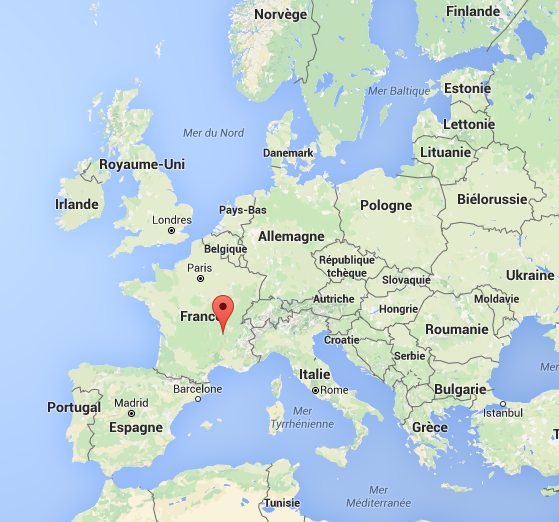
\includegraphics[height=5cm]{figures/St_Etienne}
\column{6cm}
Main area of expertise:
\begin{itemize}
	\item materials science \& mechanical engineering
	\item chemical engineering 
	\item applied mathematics, industrial engineering, environmental science
	\item biomedical and healthcare engineering
	\item microelectronics
\end{itemize}
\end{columns}
\end{frame}

%%%%%%%%%%%%%%%%%%%%%%%%%%%%%%%%%%%%%%%%%%%%%%%%%%%%%%
\begin{frame}{}
\begin{center}
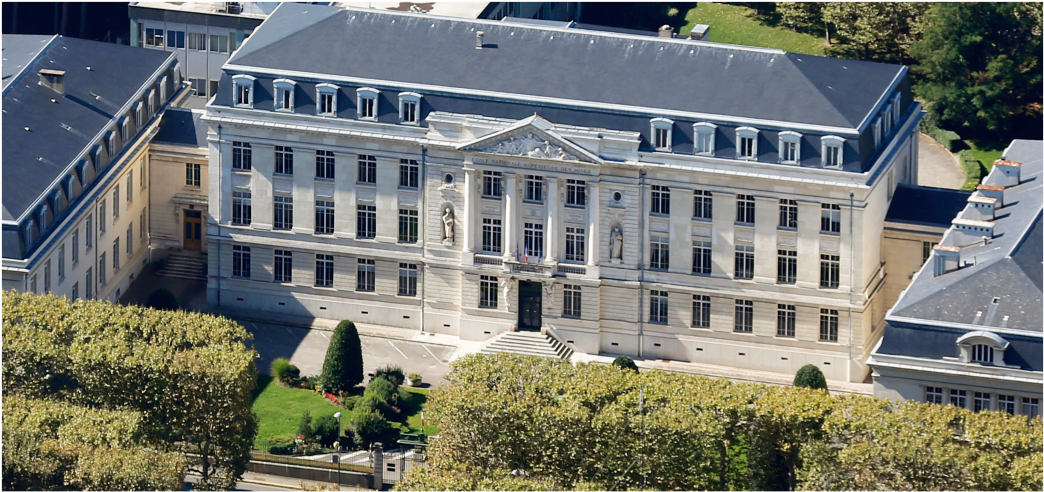
\includegraphics[height=4cm]{figures/Mines}
\end{center}
\begin{columns}[t]
\column{5cm}
\emph{Small}...
\begin{itemize}
	\item 600 students
	\item 300 faculty staff
	\item 180 PhD students 
\end{itemize}
\column{5cm}
but \emph{famous}: it is one of the leading French ``grandes écoles''.\\
\end{columns}
\vspace{5mm}
Since 2015, there is a student exchange program with the UTP.
\end{frame}

%%%%%%%%%%%%%%%%%%%%%%%%%%%%%%%%%%%%%%%%%%%%%%%%%%%%%%
\begin{frame}{}
The course will be over 4 days, with lectures every morning and lab sessions during afternoons. \\ \vspace{5mm}
The agenda is as follow:
\vspace{0.2cm}
\begin{description}
	\item[day 1:] Statistical models in engineering
	\item[day 2:] Design of experiments
	\item[day 3:] Gaussian Process regression
	\item[day 4:] Optimization  with Gaussian Process Regression
\end{description}
\vspace{5mm}
The course material is available
\begin{itemize}
	\item[] webpage: {\small https://sites.google.com/site/nicolasdurrandehomepage}
	\item[] github: {\small user NicolasDurrande, repo Gaussian-Processes-short-Course}
\end{itemize}

\end{frame}

%%%%%%%%%%%%%%%%%%%%%%%%%%%%%%%%%%%%%%%%%%%%%%%%%%%%%%
\begin{frame}{}
The lab session will be on the optimization of a catapult simulator:\\
 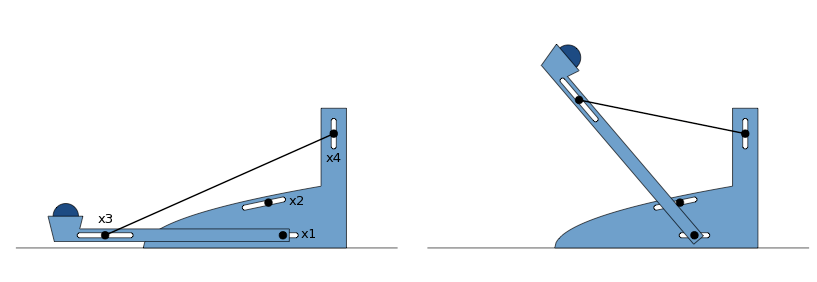
\includegraphics[width=\textwidth]{figures/Catapult}
 \vspace{0.5mm}
\vspace{4mm}
\begin{center}
	\textbf{What values of $(x_1,\ x_2,\ x_3,\ x_4)$ give the longest throw?}
\end{center}
\end{frame}

%%%%%%%%%%%%%%%%%%%%%%%%%%%%%%%%%%%%%%%%%%%%%%%%%%%%%%
\begin{frame}{}
This lab is based on a numerical simulator. Although the problem is simplistic, it shares a lot with classical engineering problems:
\begin{itemize}
	\item Black box simulator $\rightarrow$ no analytical solution
	\item Noisy response (we will be interested in the breesy wind conditions)
	\item Experiments are ``costly'' $\rightarrow$ data is limited
	\item ``High dimensional'' input space $\rightarrow$ graphical interpretation is not possible
\end{itemize}
\end{frame}

%%%%%%%%%%%%%%%%%%%%%%%%%%%%%%%%%%%%%%%%%%%%%%%%%%%%%%
\begin{frame}{}
The project will be over 4 lab sessions:
\vspace{2mm}
\begin{itemize}
	\item \textbf{Day 1:} data analysis, problem parametrization, region of interest
	\item \textbf{Day 2:} Design of experiments, data generation
	\item \textbf{Day 3:} statistical modelling
	\item \textbf{Day 4:} Optimization, new experiments
\end{itemize}
Lab sessions will be in python.
\vspace{5mm}
\begin{center}
	Make sure you bring computers !
\end{center}
\end{frame}

%%%%%%%%%%%%%%%%%%%%%%%%%%%%%%%%%%%%%%%%%%%%%%%%%%%%%%
\begin{frame}{}
Outline of today's lecture
\vspace{0.2cm}
\begin{itemize}
	\item Why (and when) statistical models can be useful in engineering?
	\item A basic example: Linear regression.
	\item Gaussian process regression
\end{itemize}
\end{frame}

%%%%%%%%%%%%%%%%%%%%%%%%%%%%%%%%%%%%%%%%%%%%%%%%%%%%%%
%%%%%%%%%%%%%%%%%%%%%%%%%%%%%%%%%%%%%%%%%%%%%%%%%%%%%%
\section[Context]{Why are statistical models relevant in engineering?}
\subsection{}

%%%%%%%%%%%%%%%%%%%%%%%%%%%%%%%%%%%%%%%%%%%%%%%%%%%%%%
\begin{frame}{}
There is a wide variety of situations where getting data about a system performance can be extremely expensive.
\begin{itemize}
	\item real world experiments
	\item destructive tests
	\item prototyping
	\item numerical experiments
\end{itemize}
\end{frame}

%%%%%%%%%%%%%%%%%%%%%%%%%%%%%%%%%%%%%%%%%%%%%%%%%%%%%%
\begin{frame}{}
\begin{exampleblock}{Example: real world experiments}
\begin{center}
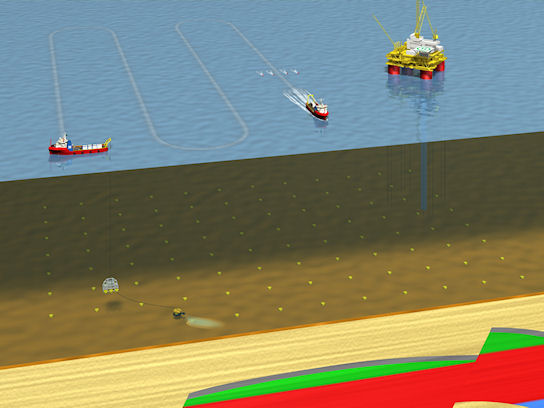
\includegraphics[height=5cm]{figures/drilling}
\end{center}
\end{exampleblock}
\end{frame}

%%%%%%%%%%%%%%%%%%%%%%%%%%%%%%%%%%%%%%%%%%%%%%%%%%%%%%
\begin{frame}{}
\begin{exampleblock}{Example: Destructive tests}
\begin{center}
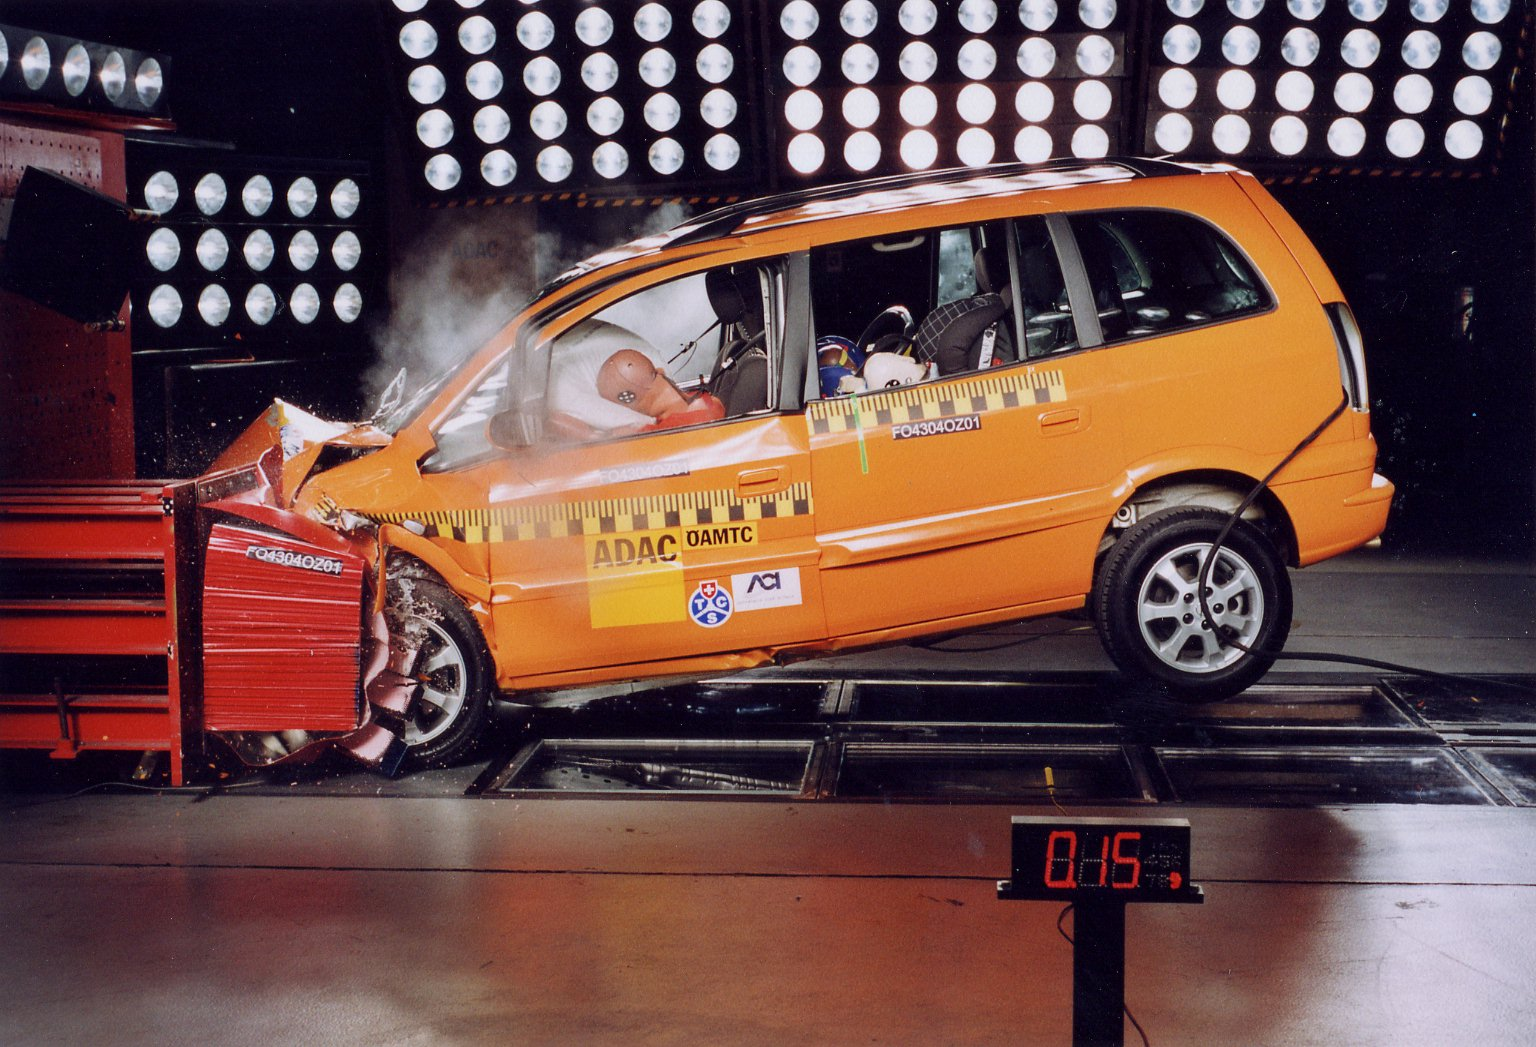
\includegraphics[height=5cm]{figures/crash-test}
\end{center}
\end{exampleblock}
\end{frame}

%%%%%%%%%%%%%%%%%%%%%%%%%%%%%%%%%%%%%%%%%%%%%%%%%%%%%%
\begin{frame}{}
\begin{exampleblock}{Example: Prototyping of a boat shape}
\begin{center}
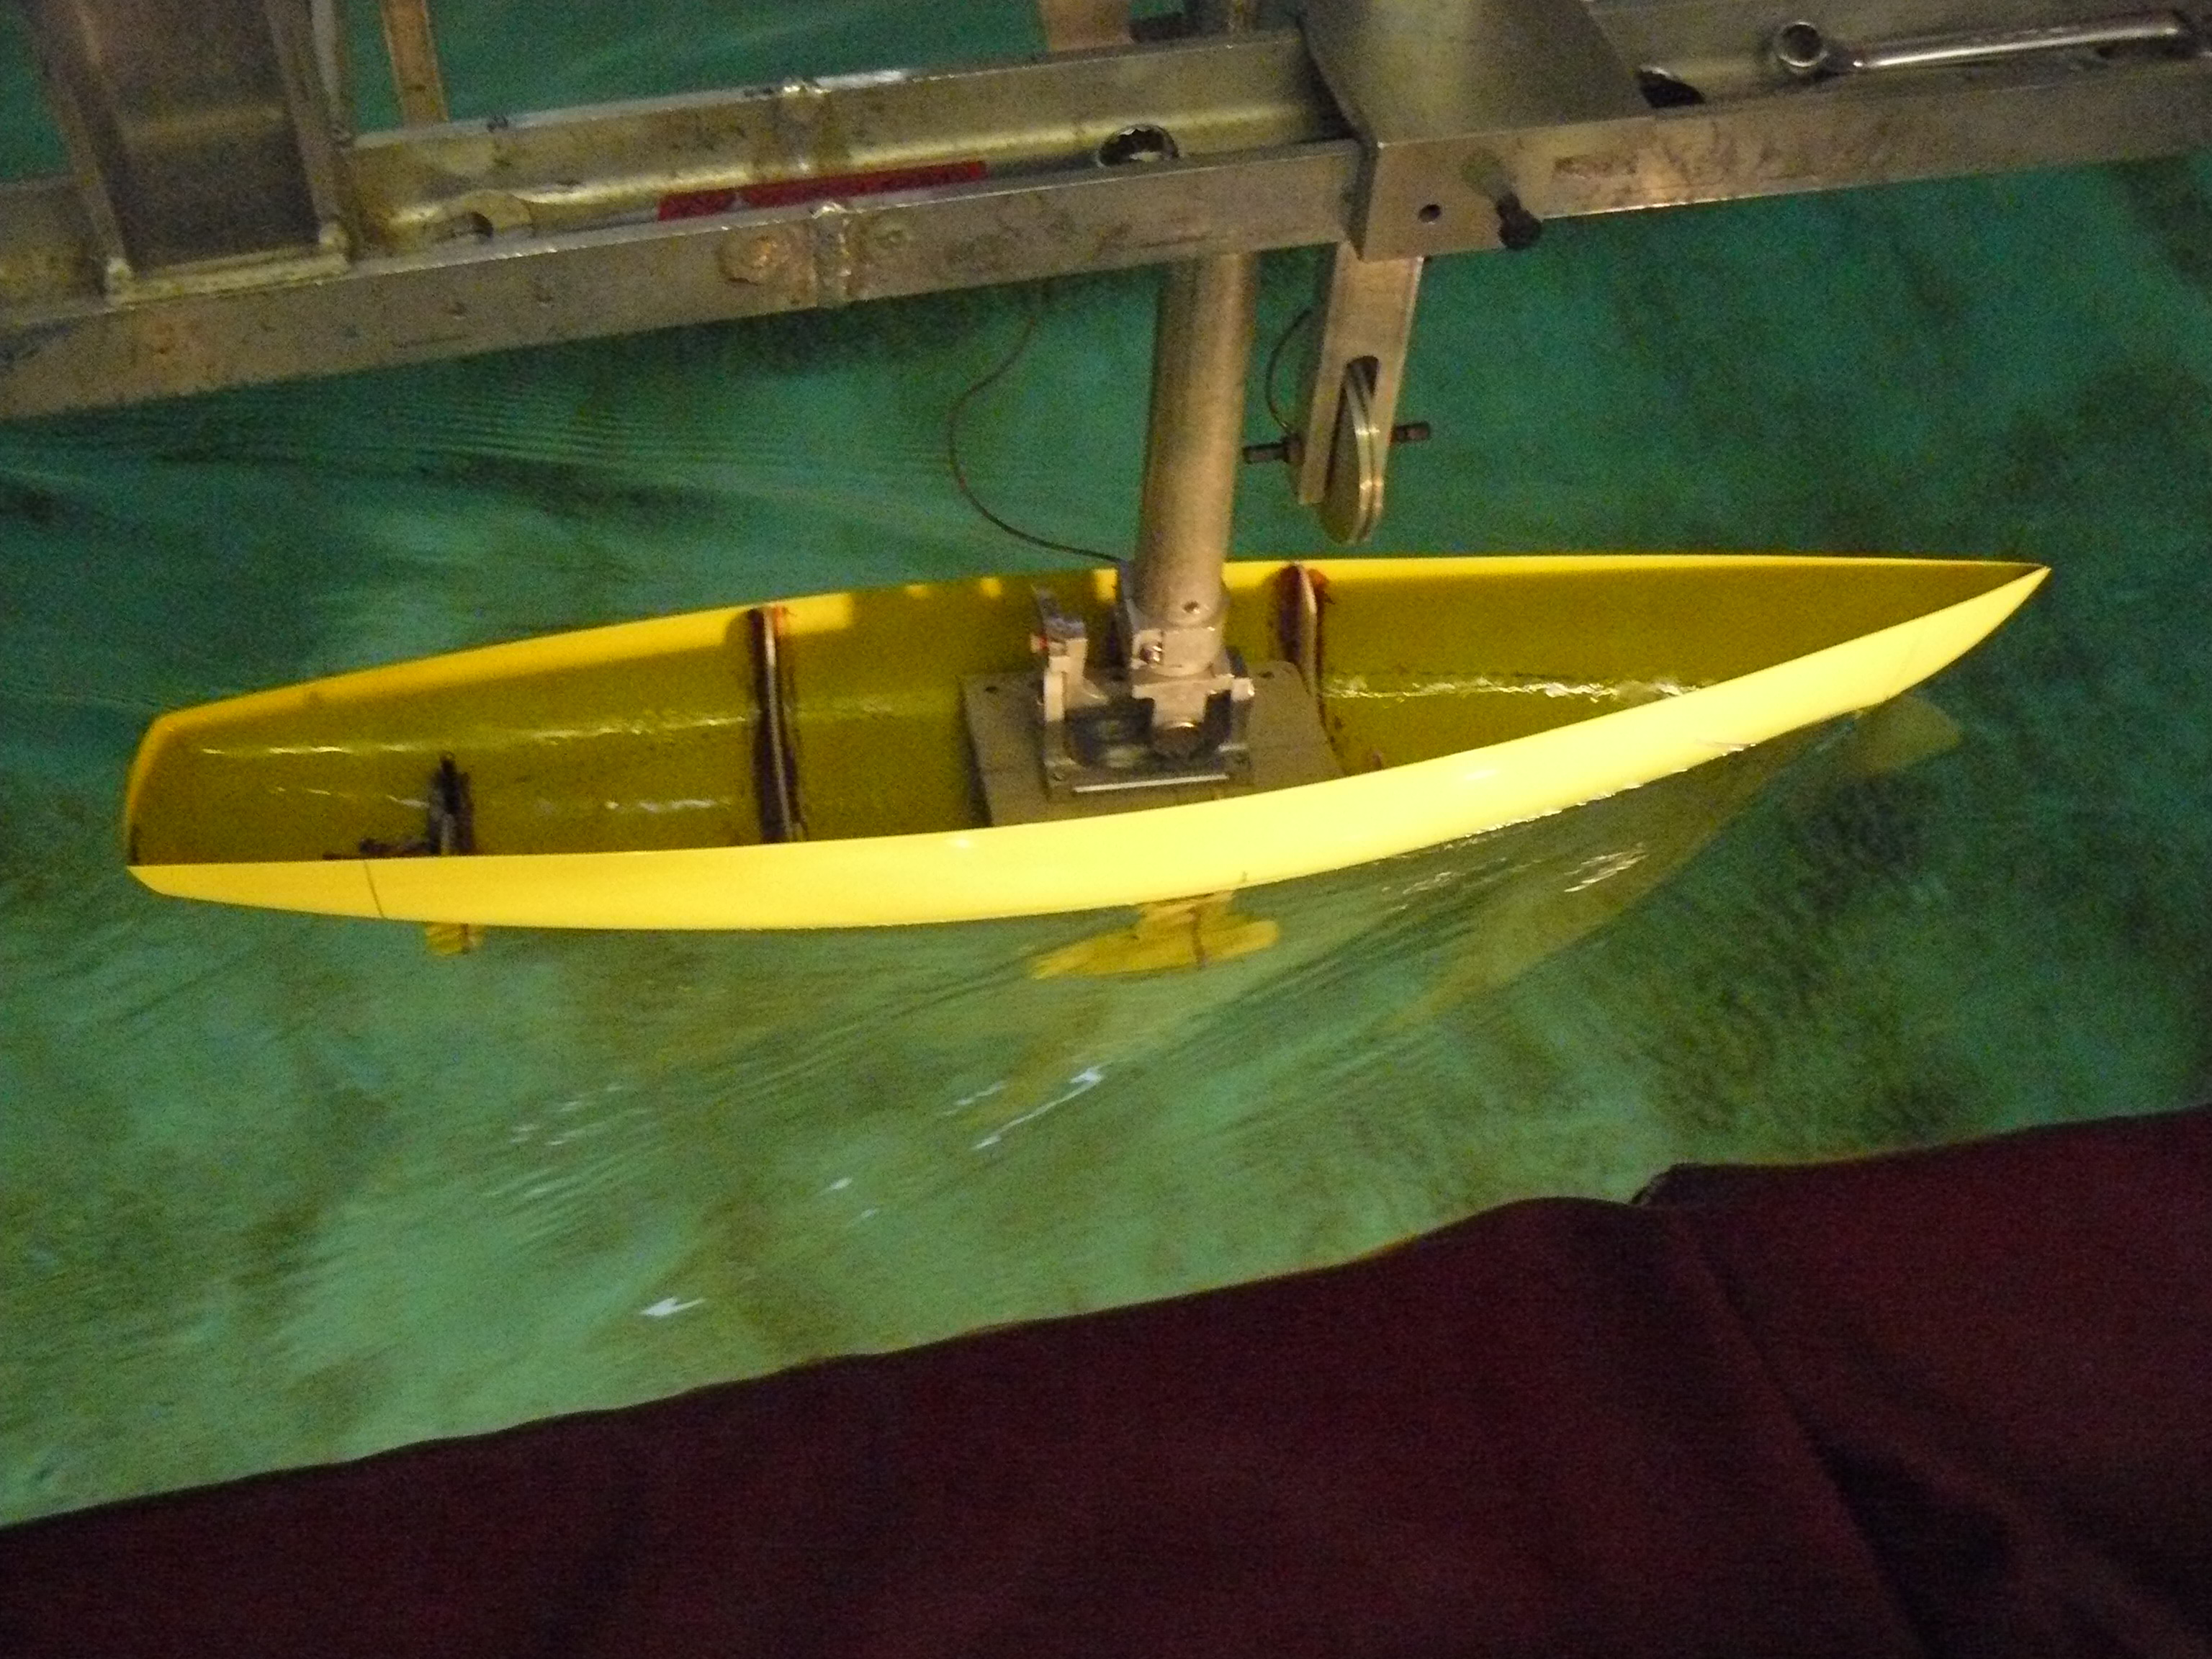
\includegraphics[height=3.5cm]{figures/carene} \qquad 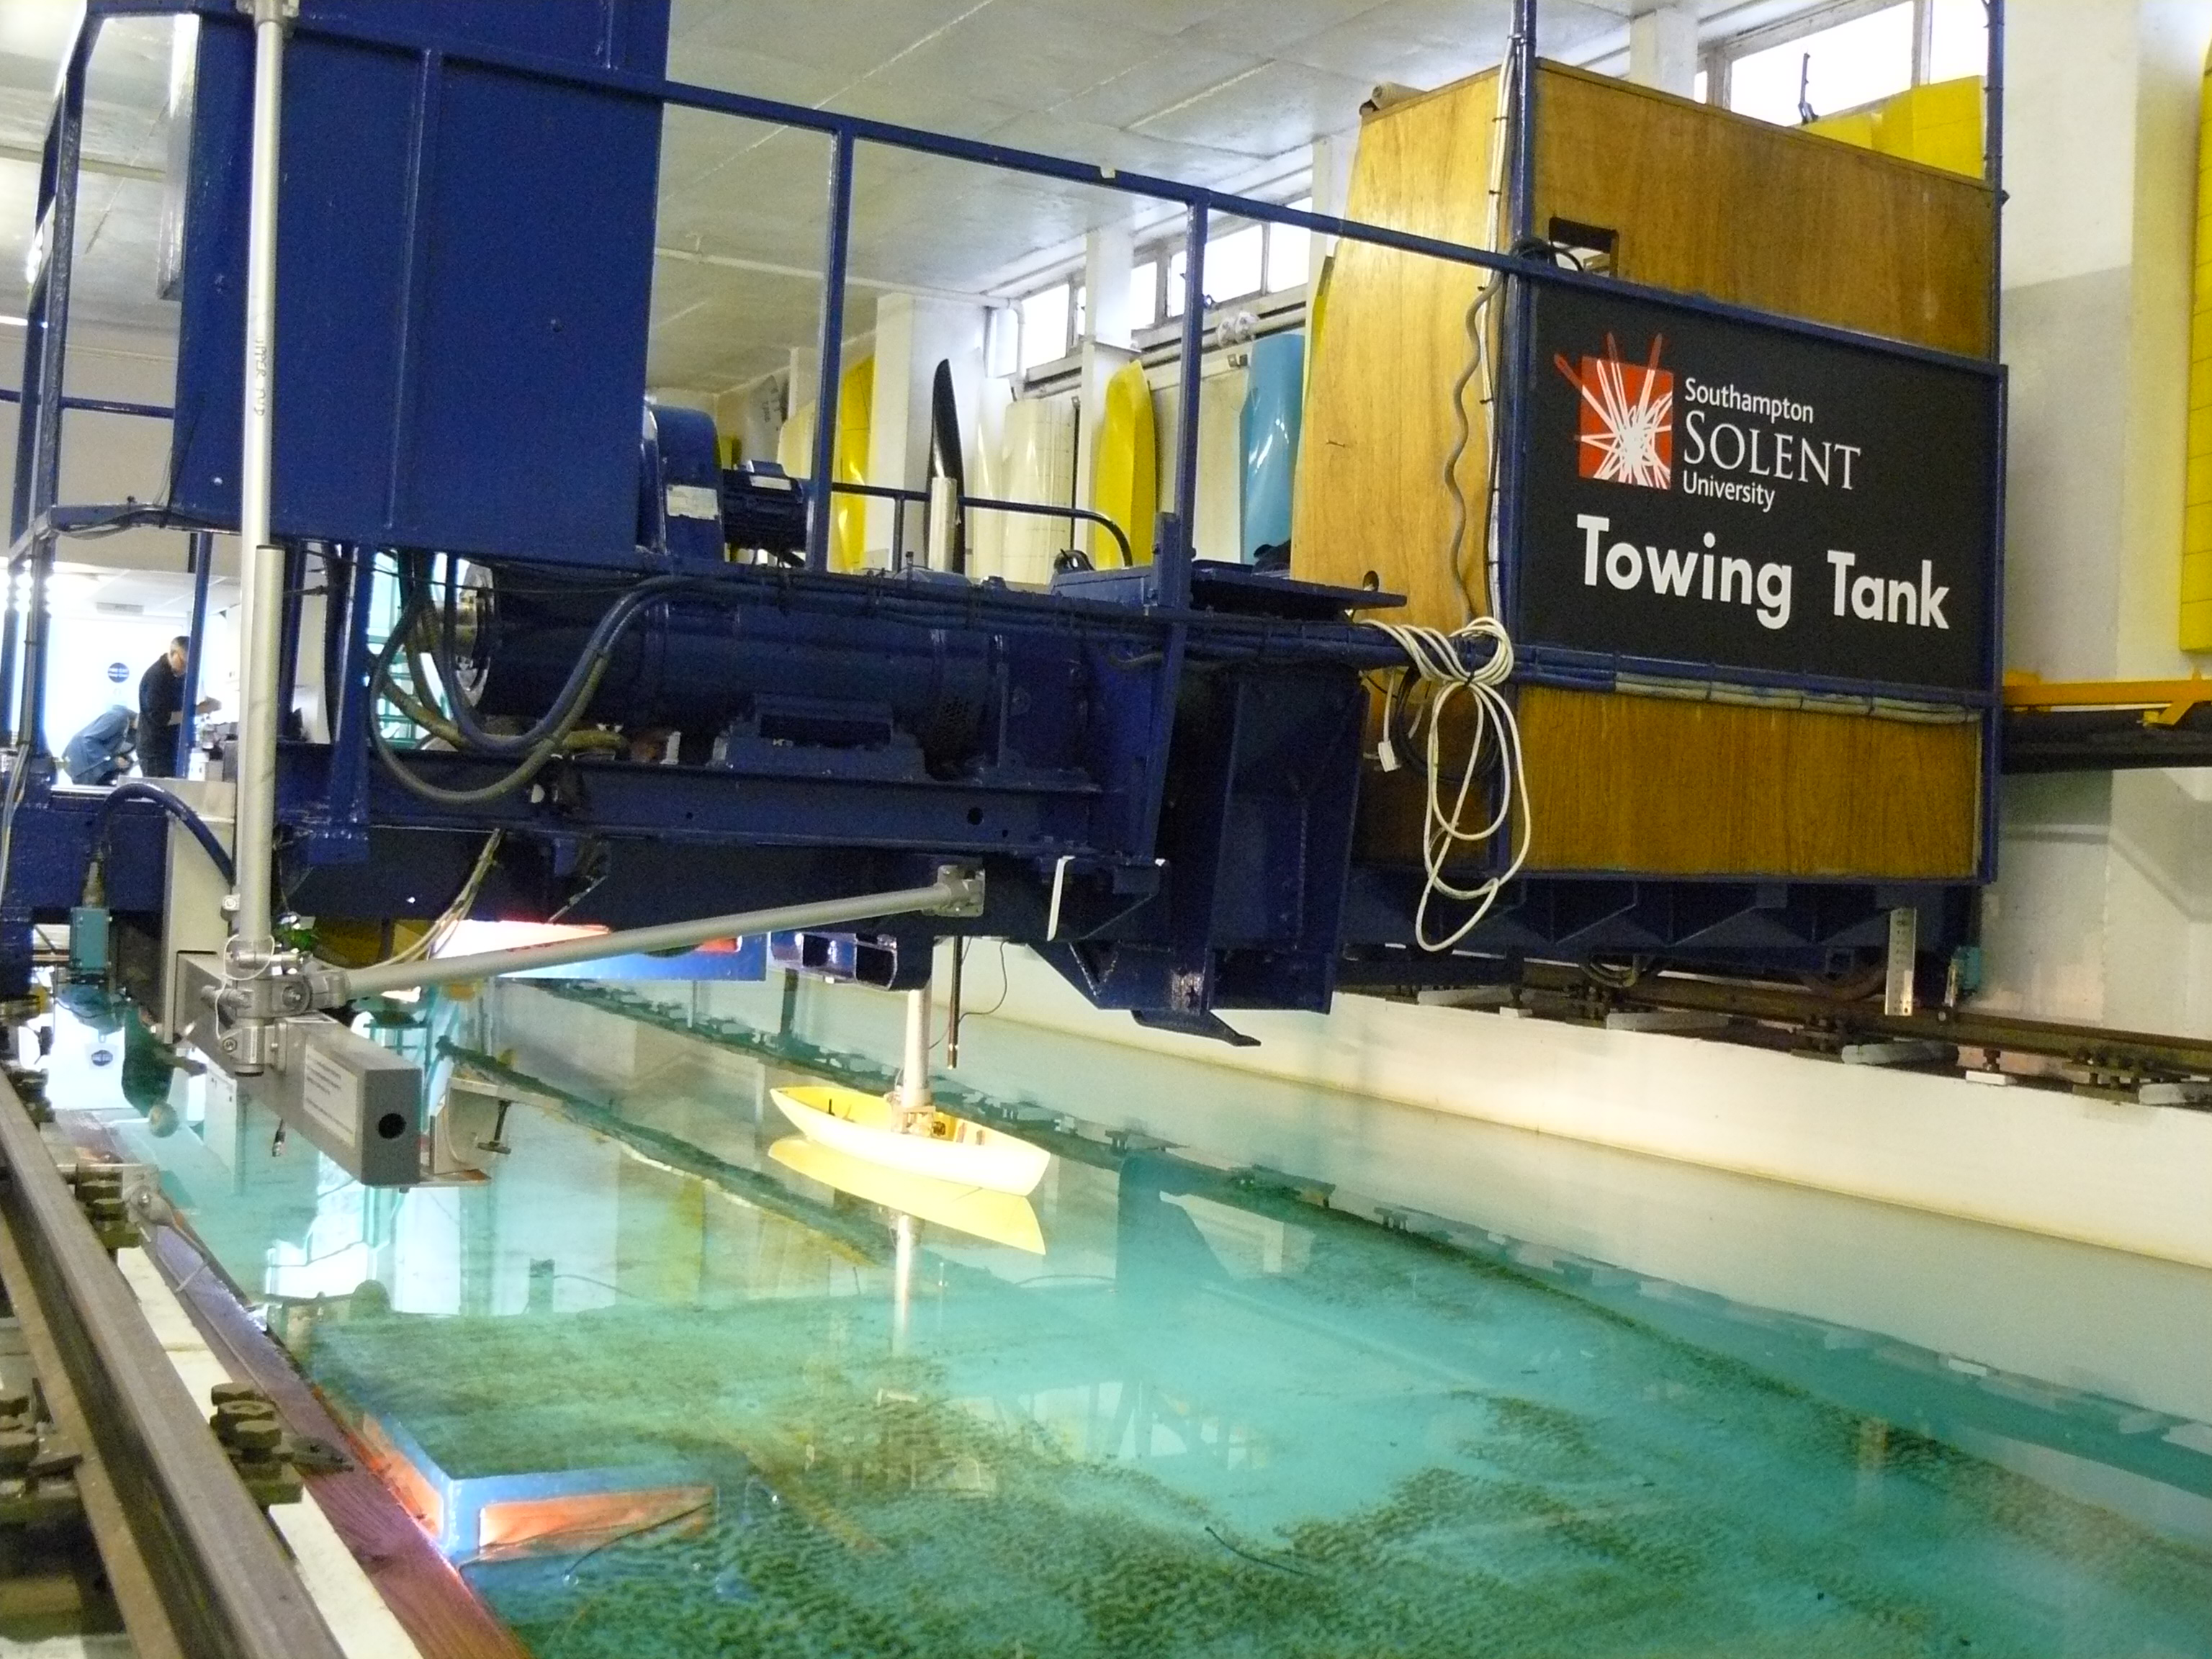
\includegraphics[height=3.5cm]{figures/carene2}
\end{center}
Knowing the drag for a given design requires costly experiments
\end{exampleblock}
\end{frame}

%%%%%%%%%%%%%%%%%%%%%%%%%%%%%%%%%%%%%%%%%%%%%%%%%%%%%%
\begin{frame}{}
\begin{exampleblock}{Example: Numerical experiments}
\begin{center}
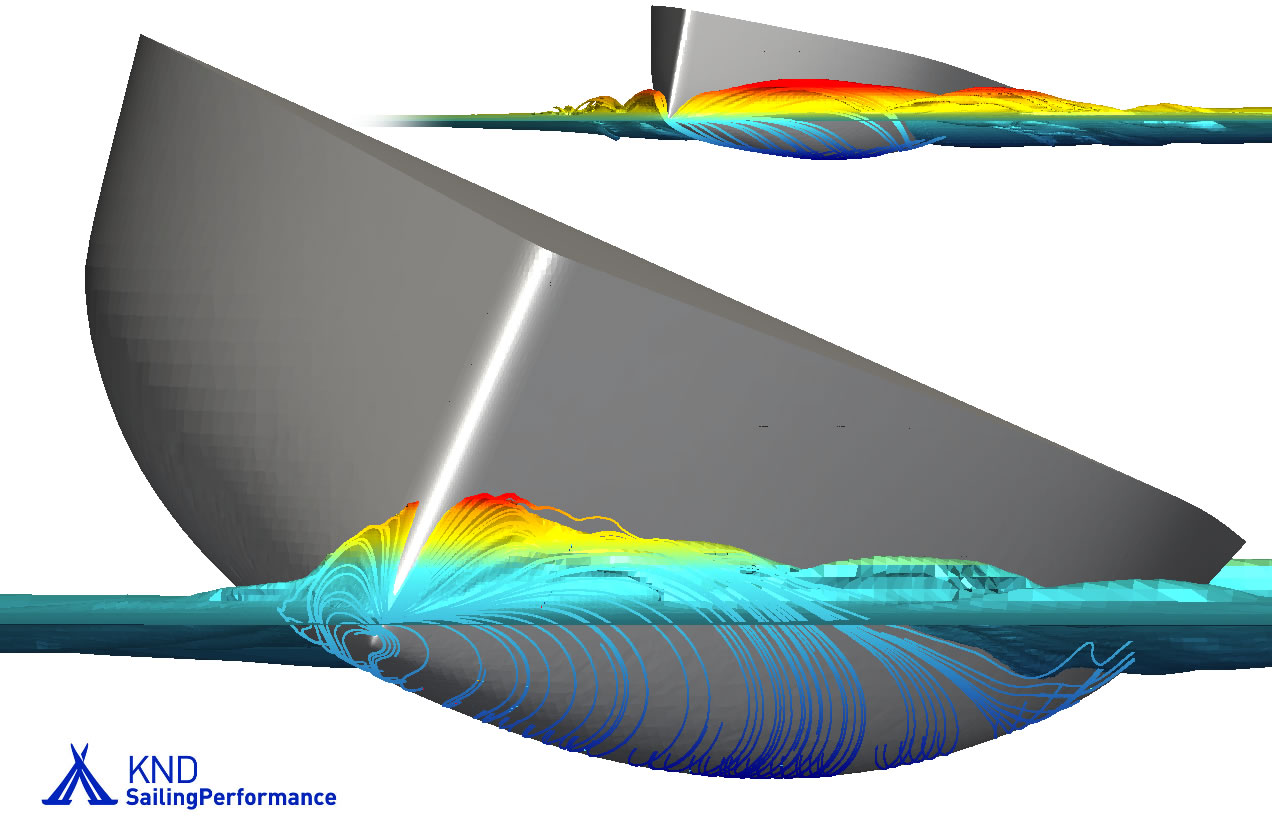
\includegraphics[height=2.8cm]{figures/waterflow} \qquad 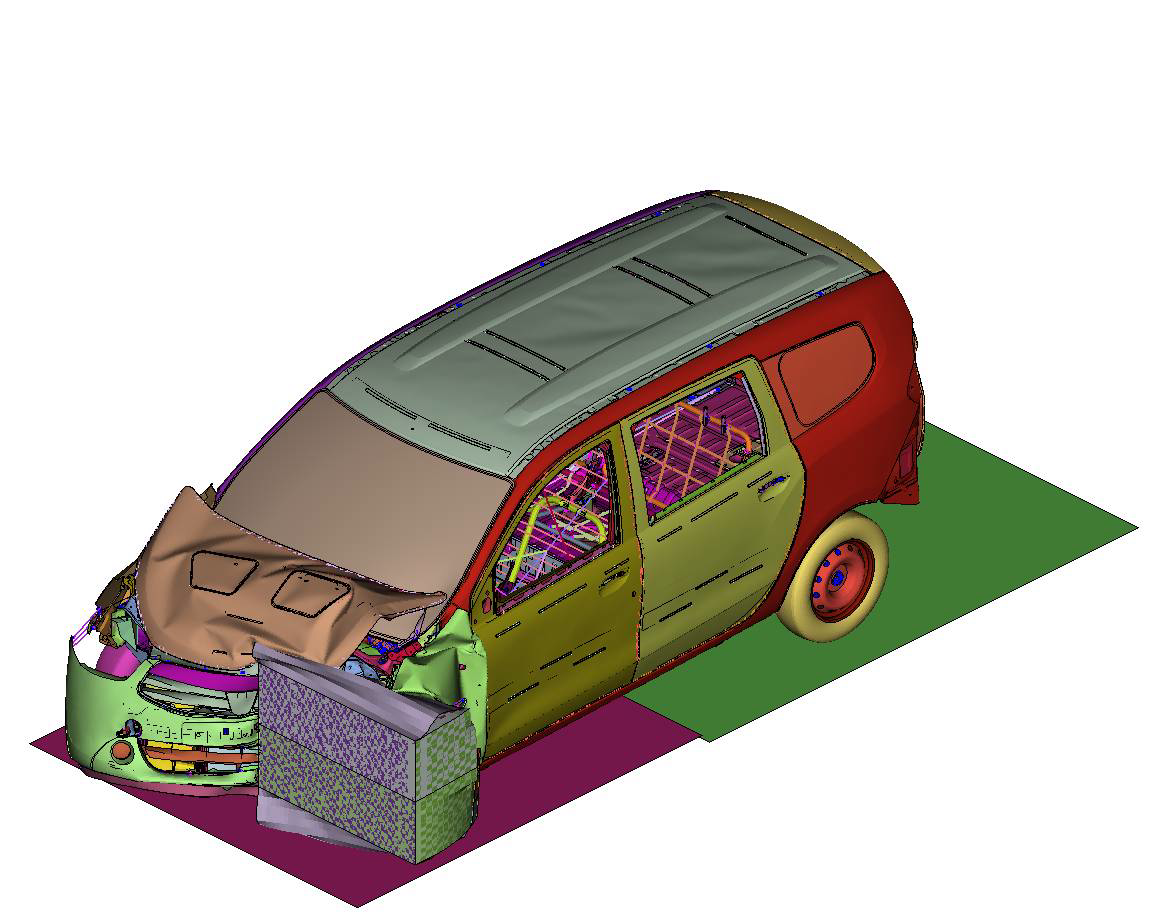
\includegraphics[height=4.2cm]{figures/crash/image15}
\end{center}
Numerical experiments are less expensive but can be very time consuming!
\end{exampleblock}
\end{frame}

%%%%%%%%%%%%%%%%%%%%%%%%%%%%%%%%%%%%%%%%%%%%%%%%%%%%%%
\begin{frame}{}
In all these cases, the variable of interest can be seen as a function of the input parameters
$$ y = f(x). $$
where $f$ is a \textbf{costly to evaluate function}. \\
\vspace{5mm}
In the following, we will assume that 
\begin{itemize}
	\item $x \in \mathds{R}^d$: There are many input parameters
	\item $y \in \mathds{R}$: The output is a scalar.
\end{itemize}
\end{frame}

%%%%%%%%%%%%%%%%%%%%%%%%%%%%%%%%%%%%%%%%%%%%%%%%%%%%%%
\begin{frame}{}
The fact that $f$ is \textbf{costly to evaluate} changes a lot of things...\\
\vspace{5mm}
\structure{1. Representing the function is not possible...}\\
\vspace{5mm}
\begin{center}
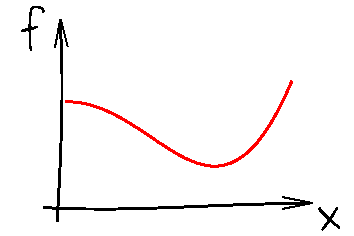
\includegraphics[height=3.2cm]{figures/ink_f} 
\includegraphics[height=3.2cm]{figures/Rightarrow} 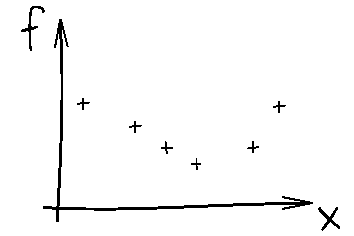
\includegraphics[height=3.2cm]{figures/ink_fX}
\end{center}
\end{frame}

%%%%%%%%%%%%%%%%%%%%%%%%%%%%%%%%%%%%%%%%%%%%%%%%%%%%%%
\begin{frame}{}
The fact that $f$ is \textbf{costly to evaluate} changes a lot of things...\\
\vspace{5mm}
\structure{2. Computing integrals is not possible...}\\
\vspace{5mm}
\begin{center}
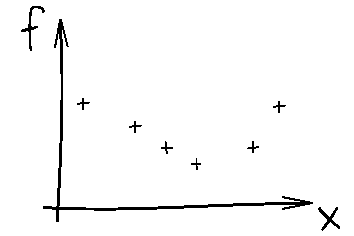
\includegraphics[height=4.5cm]{figures/ink_fX}
\end{center}
What is the mean value of $f$?
\end{frame}

%%%%%%%%%%%%%%%%%%%%%%%%%%%%%%%%%%%%%%%%%%%%%%%%%%%%%%
\begin{frame}{}
The fact that $f$ is \textbf{costly to evaluate} changes a lot of things...\\
\vspace{5mm}
\structure{3. Uncertainty propagation is not possible...}\\
\vspace{5mm}
\begin{center}
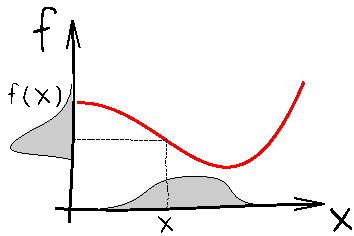
\includegraphics[height=3.2cm]{figures/ink_unprogf} 
\includegraphics[height=3.2cm]{figures/Rightarrow} 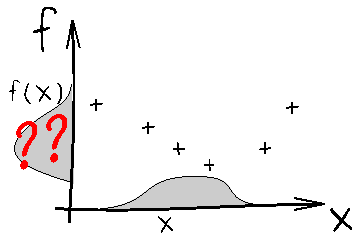
\includegraphics[height=3.2cm]{figures/ink_unprogfX}
\end{center}
\end{frame}

%%%%%%%%%%%%%%%%%%%%%%%%%%%%%%%%%%%%%%%%%%%%%%%%%%%%%%
\begin{frame}{}
The fact that $f$ is \textbf{costly to evaluate} changes a lot of things...\\
\vspace{5mm}
\structure{4. Sensitivity analysis is not possible...}\\
\vspace{5mm}
\begin{center}
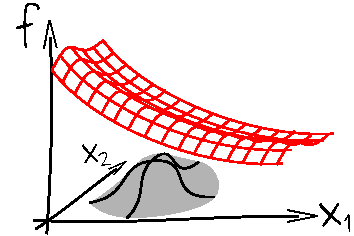
\includegraphics[height=4.5cm]{figures/ink_as}
\end{center}
\end{frame}

%%%%%%%%%%%%%%%%%%%%%%%%%%%%%%%%%%%%%%%%%%%%%%%%%%%%%%
\begin{frame}{}
The fact that $f$ is \textbf{costly to evaluate} changes a lot of things...\\
\vspace{5mm}
\structure{5. Optimisation is also tricky...}\\
\vspace{5mm}
\begin{center}
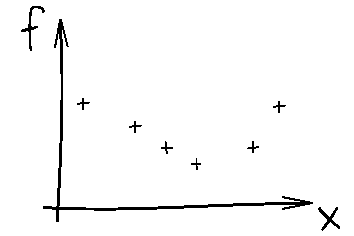
\includegraphics[height=4.5cm]{figures/ink_fX}
\end{center}
\end{frame}

%%%%%%%%%%%%%%%%%%%%%%%%%%%%%%%%%%%%%%%%%%%%%%%%%%%%%%
%%%%%%%%%%%%%%%%%%%%%%%%%%%%%%%%%%%%%%%%%%%%%%%%%%%%%%
\section[Statistical models]{Statistical models}
\subsection{}

%%%%%%%%%%%%%%%%%%%%%%%%%%%%%%%%%%%%%%%%%%%%%%%%%%%%%%
\begin{frame}{}
The principle of statistical modelling is to use the data to build a mathematical approximation of the function. 
\begin{center}
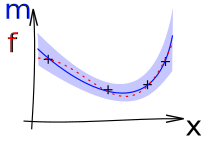
\includegraphics[height=4.5cm]{figures/ink_m}
\end{center}
The model can then be used to answer all previous questions
\end{frame}

%%%%%%%%%%%%%%%%%%%%%%%%%%%%%%%%%%%%%%%%%%%%%%%%%%%%%%
\begin{frame}{}
Of course, there is a difference between $f$ and $m$...
\begin{center}
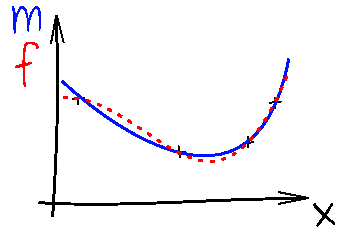
\includegraphics[height=5cm]{figures/ink_mf}
\end{center}
\end{frame}

%%%%%%%%%%%%%%%%%%%%%%%%%%%%%%%%%%%%%%%%%%%%%%%%%%%%%%
\begin{frame}{}
Why \textbf{statistical models}? \\We want to be able to quantify the model error:
\begin{center}
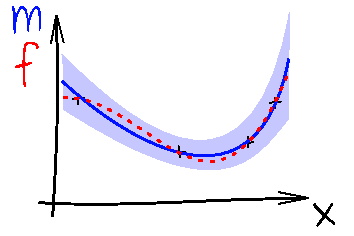
\includegraphics[height=5cm]{figures/ink_mconfint}
\end{center}
The confidence intervals can be used to obtain a \textbf{measure of uncertainty on the value of interest}.
\end{frame}

%%%%%%%%%%%%%%%%%%%%%%%%%%%%%%%%%%%%%%%%%%%%%%%%%%%%%%
\begin{frame}{}
In the sequel, we will use the following notations : 
\begin{itemize}
	\item The set of observation points will be represented by a $n \times d$ matrix $X=(X_1, ..., X_n)^t$
	\item The vector of observations will be denoted by $F$ : $F_i=f(X_i)$ (or $F=f(X)$).
\end{itemize}
We will now discuss two types of statistical models:
\begin{itemize}
	\item Linear regression
	\item Gaussian process regression
\end{itemize}
\end{frame}

%%%%%%%%%%%%%%%%%%%%%%%%%%%%%%%%%%%%%%%%%%%%%%%%%%%%%%
%%%%%%%%%%%%%%%%%%%%%%%%%%%%%%%%%%%%%%%%%%%%%%%%%%%%%%
\section{Linear Regression}
\subsection{}

%%%%%%%%%%%%%%%%%%%%%%%%%%%%%%%%%%%%%%%%%%%%%%%%%%%%%%
\begin{frame}{}
\textbf{Linear regression} is probably the most commonly used statistical model.\\ \vspace{3mm}
Given a set of basis functions $B=(b_0, \dots, b_p)$, we assume that the observations come from the probabilistic model
$$ F = B(X) \beta  + \varepsilon \qquad \qquad \left( \text{i.e. } F_i = \sum_{k=1}^p \beta_k b_k(X_i) + \varepsilon_i \right) $$
where the vector $\beta$ is unknown, $\varepsilon_i$ are independent and identically distributed and
$$ B(X)_{(i,j)}=b_j(X_i) $$
\end{frame}

%%%%%%%%%%%%%%%%%%%%%%%%%%%%%%%%%%%%%%%%%%%%%%%%%%%%%%
\begin{frame}{}
If we consider a model of the form 
$$m(x) = B(x) \hat{\beta}$$
the prediction error (Residual Sum of Square) is given by 
$$RSS = (B(X) \hat{\beta}  - F)^t(\hat{\beta} B(X) - F)  \qquad \qquad \left( \text{i.e. } \sum_{k=1}^n ( B(X_i) \hat{\beta} - F_i)^2\right)$$ 

Finding the optimal value of $\hat{\beta}$ means minimizing a quadratic form. This can be done analytically and we obtain $\hat{\beta} = (B(X)^t B(X))^{-1} B(X)^t F$.\\
\vspace{3mm}
The associated linear regression model is thus
$$m(x) = B(x) (B(X)^t B(X))^{-1} B(X)^t F.$$
\end{frame}

%%%%%%%%%%%%%%%%%%%%%%%%%%%%%%%%%%%%%%%%%%%%%%%%%%%%%%
\begin{frame}{}
\begin{example}
	If we consider the following observations: 
\begin{center}
  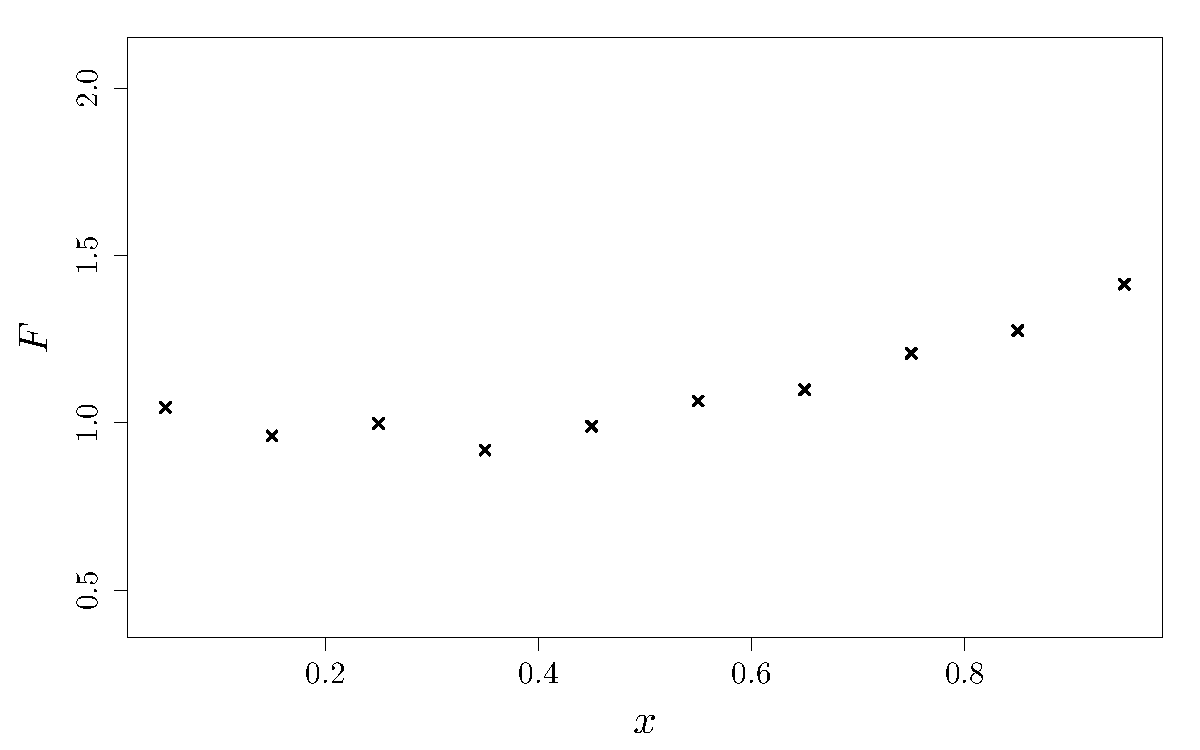
\includegraphics[height=5cm]{figures/R/linreg_0}
\end{center}
\end{example}
\end{frame}

%%%%%%%%%%%%%%%%%%%%%%%%%%%%%%%%%%%%%%%%%%%%%%%%%%%%%%
\begin{frame}{}
\begin{example}
	and a set of 3 basis functions:
	 $$b_0(x)=1,\ b_1(x)=x,\ b_2(x)=x^2$$
\begin{center}
  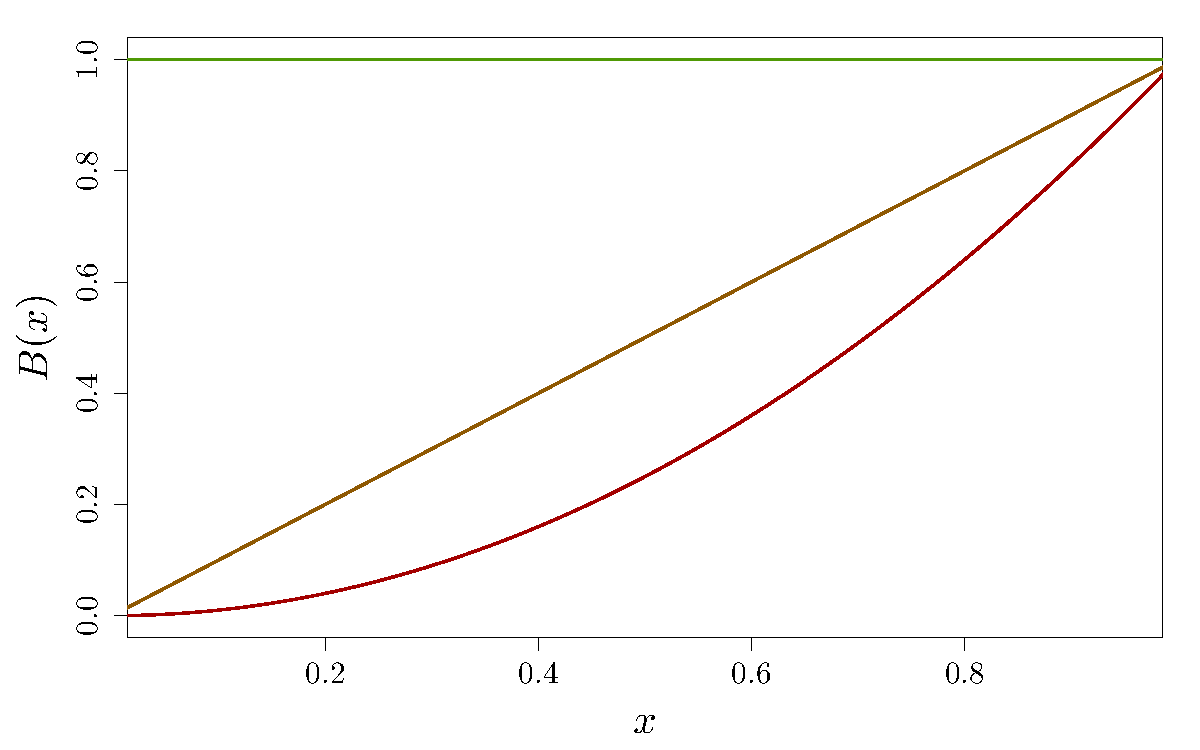
\includegraphics[height=5cm]{figures/R/linreg_1}
\end{center}
\end{example}
\end{frame}

%%%%%%%%%%%%%%%%%%%%%%%%%%%%%%%%%%%%%%%%%%%%%%%%%%%%%%
\begin{frame}{}
\begin{example}
We obtain $\hat{\beta} = (1.06,-0.61,1.04)$ and the model is:
\begin{center}
  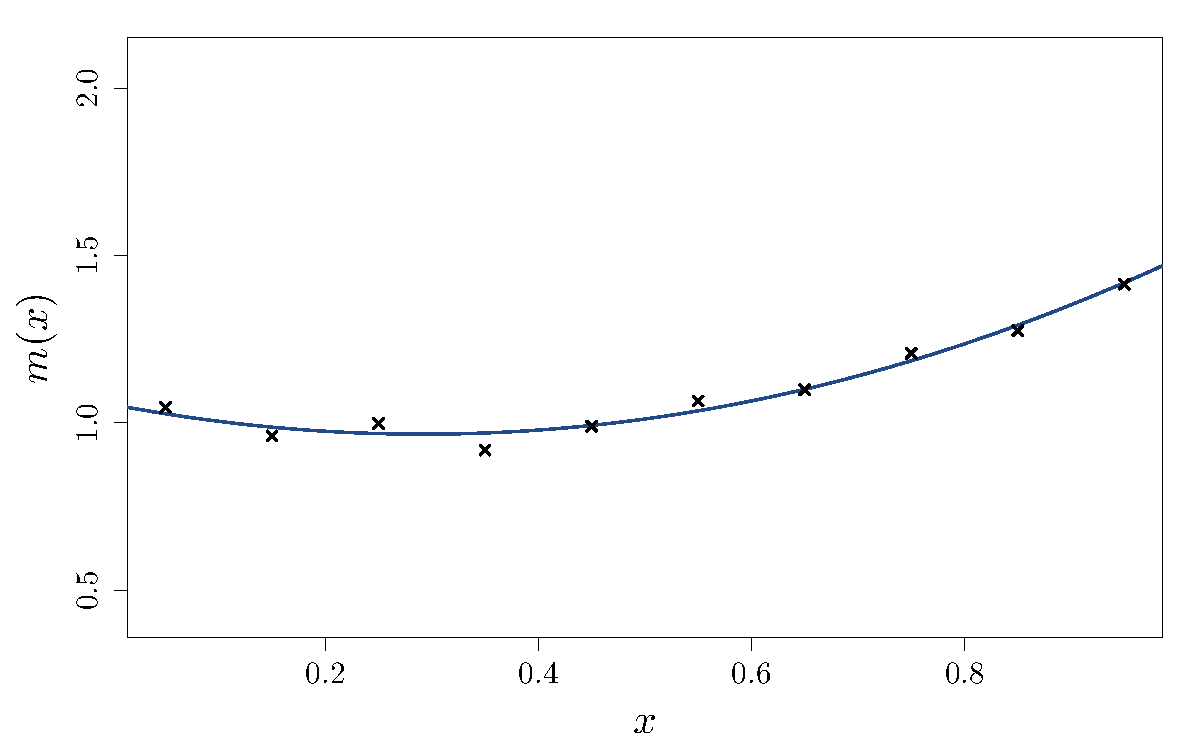
\includegraphics[height=5cm]{figures/R/linreg_2}
\end{center}
\end{example}
\end{frame}

%%%%%%%%%%%%%%%%%%%%%%%%%%%%%%%%%%%%%%%%%%%%%%%%%%%%%%
\begin{frame}{}
\begin{example}
There is of course an error between the true generative function and the model
\begin{center}
  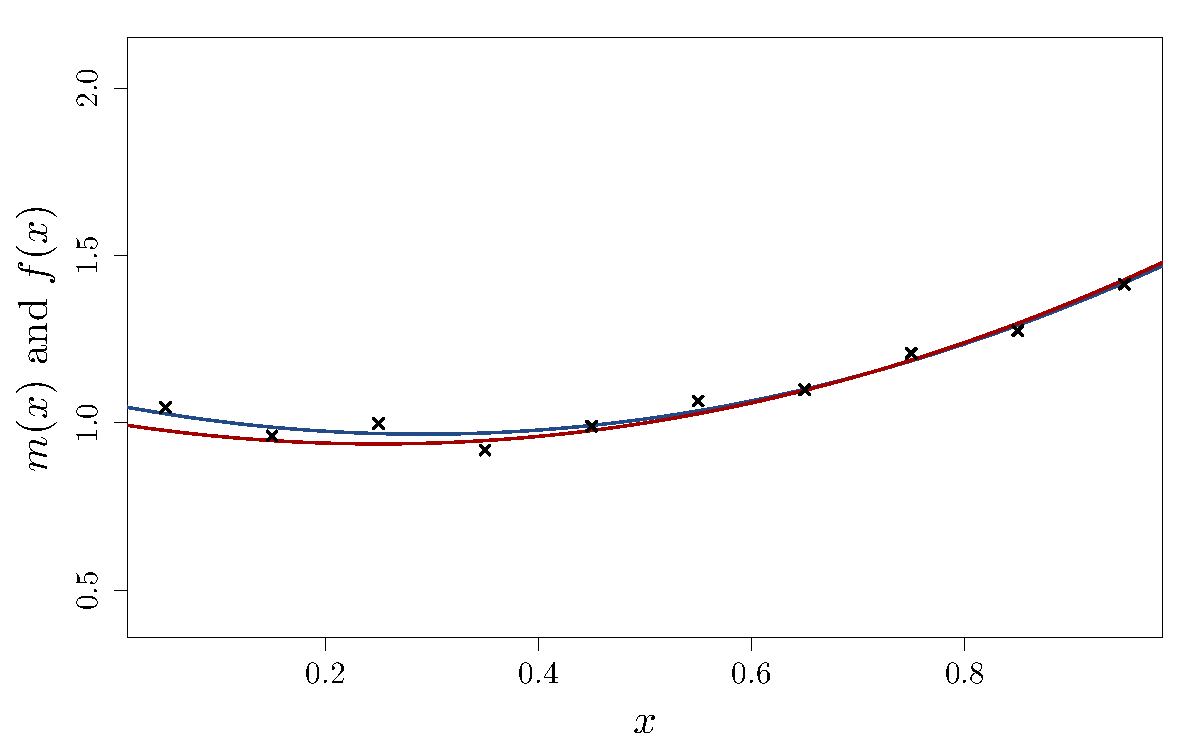
\includegraphics[height=5cm]{figures/R/linreg_3}
\end{center}
Can this error be quantified?
\end{example}
\end{frame}

%%%%%%%%%%%%%%%%%%%%%%%%%%%%%%%%%%%%%%%%%%%%%%%%%%%%%%
\begin{frame}{}
The initial assumption is $ F = B(X) \beta  + \varepsilon$ and we have computed an estimator of $\beta$:
$$\hat{\beta} = (B(X)^t B(X))^{-1} B(X)^t F.$$
$\hat{\beta}$ can thus be seen as a sample from the random variable:
$$\hat{\beta} = (B(X)^t B(X))^{-1} B(X)^t (B(X) \beta  + \varepsilon).$$ \\
\vspace{5mm}
What about the distribution of $\hat{\beta}$? \pause
\begin{itemize}
	\item Its expectation is $\beta$ \alert{$\Rightarrow$} The estimator is unbiased
	\item Its covariance matrix is $$(B(X)^t B(X))^{-1} B(X)^t \Cov[\varepsilon,\varepsilon^t] B(X) (B(X)^t B(X))^{-1}$$
	\item If $\varepsilon$ is multivariate normal, then $\hat{\beta}$ is also multivariate normal (not necessarily i.i.d.).
\end{itemize}
\end{frame}

%%%%%%%%%%%%%%%%%%%%%%%%%%%%%%%%%%%%%%%%%%%%%%%%%%%%%%
\begin{frame}{}
Sampling in the distribution of $\hat{\beta}$ gives us a large variety of models which represent the uncertainty about our estimation:
\begin{exampleblock}{Back to the example}
\begin{center}
  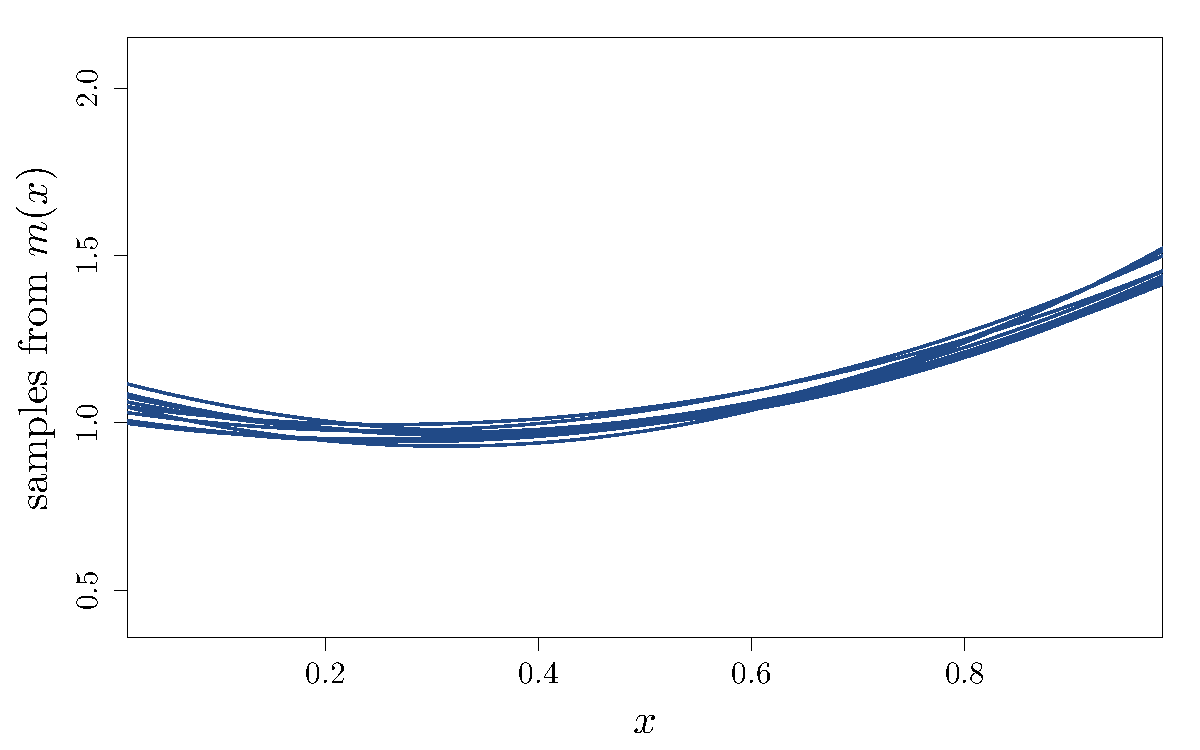
\includegraphics[height=5cm]{figures/R/linreg_4}
\end{center}
\end{exampleblock}
\end{frame}

%%%%%%%%%%%%%%%%%%%%%%%%%%%%%%%%%%%%%%%%%%%%%%%%%%%%%%
\begin{frame}{}
\begin{exampleblock}{Back to the example}
The previous picture can be summarized by showing the mean of $m$ and $95\%$ confidence intervals
\begin{center}
  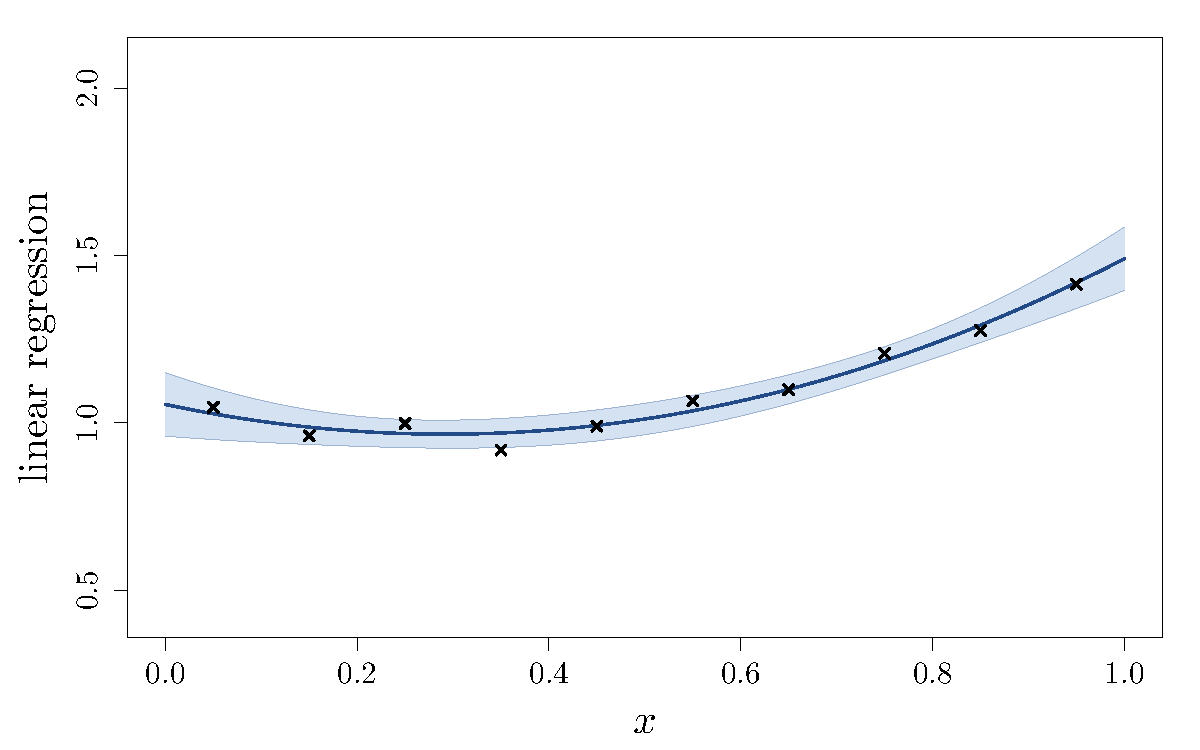
\includegraphics[height=5cm]{figures/R/linreg_5}
\end{center}
\end{exampleblock}
\end{frame}

%%%%%%%%%%%%%%%%%%%%%%%%%%%%%%%%%%%%%%%%%%%%%%%%%%%%%%
\begin{frame}{}
Knowing the uncertainty on the model allows to compute an uncertainty on the quantity of interest.
\begin{exampleblock}{Back to the example}
For example, if we are interested in the value $x^\star$ minimizing $f(x)$:
\begin{center}
  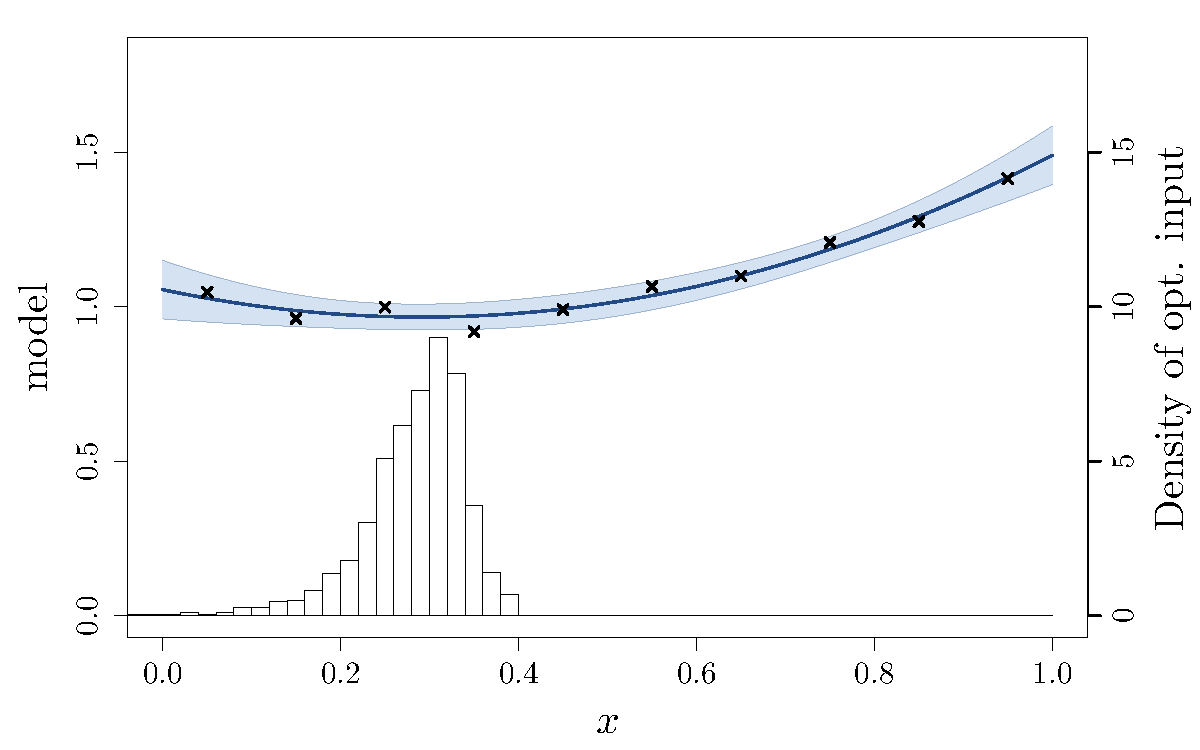
\includegraphics[height=5cm]{figures/R/linreg_6}
\end{center}
\end{exampleblock}
\alert{The expectation of $x^\star$ \textbf{is not} the input minimizing $m(x).$}
\end{frame}


%%%%%%%%%%%%%%%%%%%%%%%%%%%%%%%%%%%%%%%%%%%%%%%%%%%%%%
\begin{frame}{}
\textbf{\structure{Model validation}} is always of upper importance.\\ 
\vspace{3mm}
The goodness of fit can be measured by the \textbf{coefficient of determination}:
$$R^2 =  1 - \frac{\Var[prediction\ errors]}{\Var[data]} = 1 - \frac{\sum_i (F_i-m(X_i))^2}{\sum_i (F_i-mean(F))^2}$$
\begin{center}
  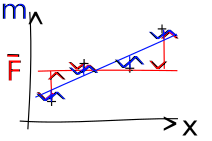
\includegraphics[height=4cm]{figures/ink_R2}
\end{center}
\alert{Be careful!} A good $R^2$ (ie close to one) does not necessarily mean that the model is good.
\end{frame}

%%%%%%%%%%%%%%%%%%%%%%%%%%%%%%%%%%%%%%%%%%%%%%%%%%%%%%
\begin{frame}{}
	We've seen that the law of $\hat{\beta}$ is multivariate Gaussian, with its covariance depending on $\varepsilon$:
	$$(B(X)^t B(X))^{-1} B(X)^t \Cov[\varepsilon,\varepsilon^t] B(X) (B(X)^t B(X))^{-1}$$
	\textbf{Ordinary regression:} suppose now $\Cov[\varepsilon,\varepsilon^t]=\sigma^2I_d$ then
	$$ \Cov[\hat{\beta},\hat{\beta}^t] = \sigma^2(B(X)^tB(X))^{-1}$$
	and from this, we now that
	$$ \frac{\hat{\beta_i}}{\sqrt{\hat{\sigma}^2(B(X)^tB(X))^{-1}_{(i,i)}}}\text{ is student}$$
	with the standard variance estimator
	$$ \hat{\sigma}^2=\frac{1}{n-p}\lVert F-m(X)\rVert^2 $$
\end{frame}


%%%%%%%%%%%%%%%%%%%%%%%%%%%%%%%%%%%%%%%%%%%%%%%%%%%%%%
\begin{frame}{}
The influence of one basis function can be tested using \textbf{p-values}:\\
\qquad $H_0$: The basis function $b_i$ has no influence (i.e. $\beta_i=0$)\\
\qquad p-values: probability of observing a larger estimate
\begin{center}
  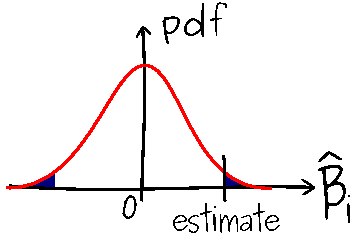
\includegraphics[height=4.5cm]{figures/ink_pvalue}
\end{center}
The smaller the p-value is, the less $\hat{\beta}$ is likely to be due to chance.
\end{frame}

%%%%%%%%%%%%%%%%%%%%%%%%%%%%%%%%%%%%%%%%%%%%%%%%%%%%%%
\begin{frame}{}
We could dedicate the entire course to linear regression models...
\begin{columns}[c]
\column{5cm}
\begin{itemize}
	\item model validation
	\item choice of basis functions
\end{itemize}
\column{6cm}
\begin{itemize}
	\item influence of input locations
	\item ...
\end{itemize}
\end{columns}
\vspace{10mm}
We will just stress a few \textbf{pros and cons of these models}:
\begin{itemize}
  \item[+] provide a good noise filtering
  \item[+] are easy to interpret
  \item[] \vspace{-5mm}
  \item[$-$] are not flexible (need to choose the basis functions)
  \item[$-$] do not interpolate
  \item[$-$] may explode when using high order polynomials (over-fitting)
\end{itemize}
\end{frame}

%%%%%%%%%%%%%%%%%%%%%%%%%%%%%%%%%%%%%%%%%%%%%%%%%%%%%%
%%%%%%%%%%%%%%%%%%%%%%%%%%%%%%%%%%%%%%%%%%%%%%%%%%%%%%
\section[Gaussian Process regression]{Gaussian Process Regression}
\subsection{}
%%%%%%%%%%%%%%%%%%%%%%%%%%%%%%%%%%%%%%%%%%%%%%%%%%%%%%
\begin{frame}{}
\vspace{0.75cm}
\structure{This section will be organised in 3 subsections:}
\vspace{0.5cm}
\begin{enumerate}
    \item Reminders on Multivariate normal distribution
    \item Gaussian processes
    \item Gaussian process regression
\end{enumerate}
\end{frame}

%%%%%%%%%%%%%%%%%%%%%%%%%%%%%%%%%%%%%%%%%%%%%%%%%%%%%%%%%%%%
%\subsection{Multivariate normal distribution}

%%%%%%%%%%%%%%%%%%%%%%%%%%%%%%%%%%%%%%%%%%%%%%%%%%%%%%
\begin{frame}{1. Multivariate normal distribution}
The usual one dimensional normal distribution $\mathcal{N}(\mu,\sigma^2)$ has the following pdf:
\begin{equation*}
f(x) = \frac{1}{\sigma \sqrt{2 \pi}} \exp \left(-\frac{(x-\mu)^2}{2 \sigma^2} \right) \text{ for } x \in \mathds{R}
\end{equation*} 
It can be generalised to vectors:
\begin{definition}
	We say that a vector $Y=(Y_1, \dots, Y_n)$ follows a multivariate normal distribution if any linear combination of $Y$ follows a normal distribution:
	\begin{equation*}
		\forall \alpha \in \mathds{R}^n,\ \alpha^t Y \sim \mathcal{N}(m,s^2)
	\end{equation*}
\end{definition}
\end{frame}

%%%%%%%%%%%%%%%%%%%%%%%%%%%%%%%%%%%%%%%%%%%%%%%%%%%%%%
\begin{frame}{}
The distribution of a Gaussian vector is characterised by
\begin{itemize}
 	\item a mean vector $\mu = (\mu_1, \dots, \mu_d)$
 	\item a $d \times d$ covariance matrix $\Sigma$ : $\Sigma_{i,j}=\Cov(Y_i, Y_j)$
\end{itemize} 
\vspace{5mm}
\structure{Property:}\\
A covariance matrix is 
\begin{itemize}
	\item \textbf{symmetric} $K_{i,j}=K_{j,i}$
	\item \textbf{positive semi-definite} $\forall \alpha \in \mathds{R}^d, \alpha^t K \alpha \geq 0$.
\end{itemize} 
\end{frame}

%%%%%%%%%%%%%%%%%%%%%%%%%%%%%%%%%%%%%%%%%%%%%%%%%%%%%%
\begin{frame}{}
The density of a multivariate Gaussian is:
\begin{equation*}
f_Y(x) = \frac{1}{\displaystyle (2 \pi)^{d/2} |\Sigma|^{1/2}} \exp \left(-\frac12 (x-\mu)^t \Sigma^{-1} (x-\mu)  \right).
\end{equation*} 
\begin{center}
 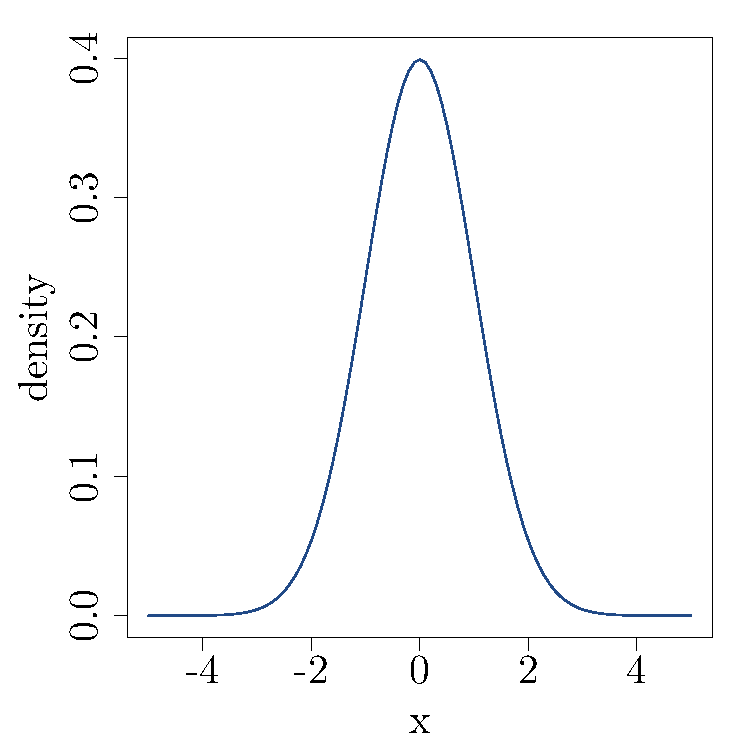
\includegraphics[height=4.7cm]{figures/R/MVN_dens1} \qquad 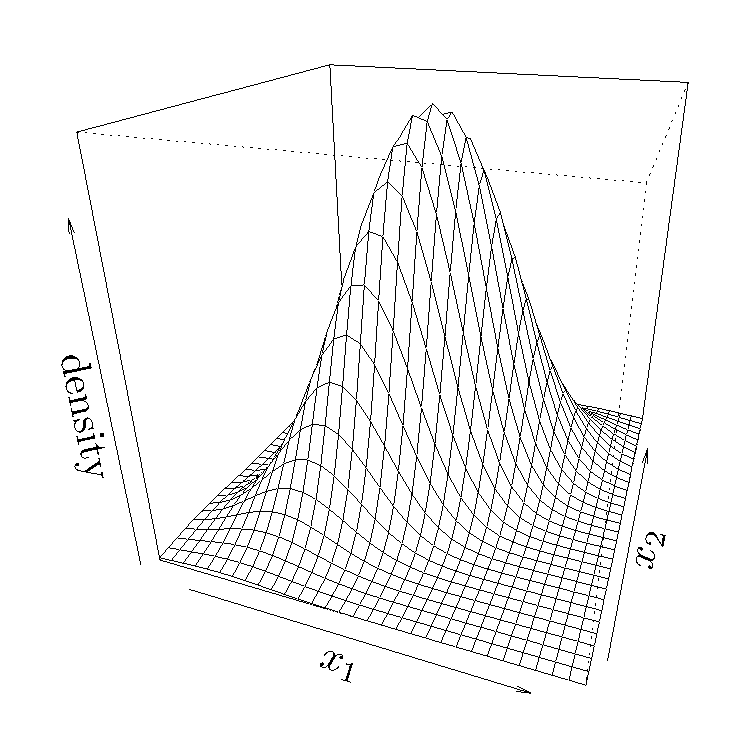
\includegraphics[height=5cm]{figures/R/MVN_dens2} 
\end{center}
\end{frame}


%%%%%%%%%%%%%%%%%%%%%%%%%%%%%%%%%%%%%%%%%%%%%%%%%%%%%%
\begin{frame}{}
\begin{example}
\begin{center}
 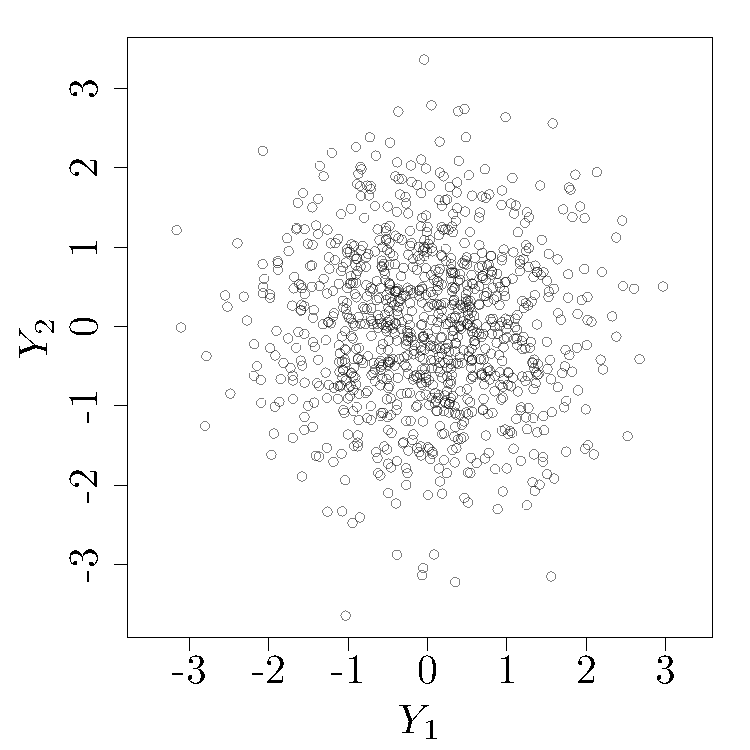
\includegraphics[height=5cm]{figures/R/MVN_gaussvec2} \quad 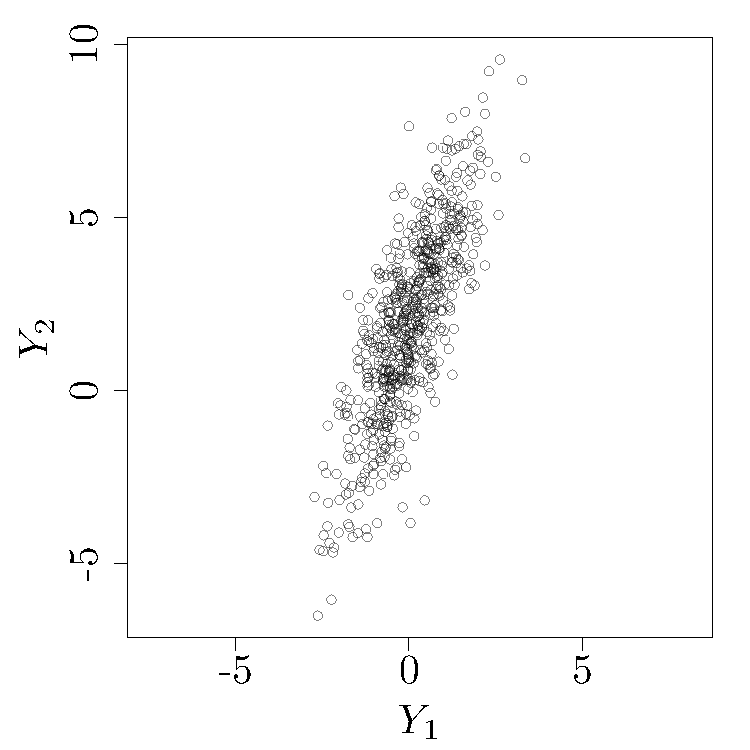
\includegraphics[height=5cm]{figures/R/MVN_gaussvec1} 
\end{center}
\end{example}
\end{frame}

%%%%%%%%%%%%%%%%%%%%%%%%%%%%%%%%%%%%%%%%%%%%%%%%%%%%%%
\begin{frame}{}
\begin{exampleblock}{Counter example}
\begin{center}
 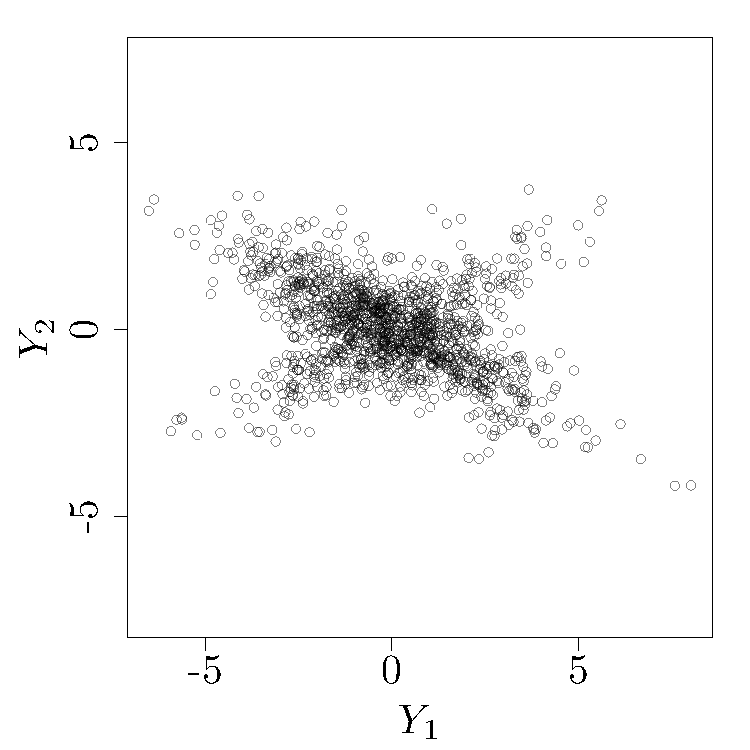
\includegraphics[height=5cm]{figures/R/MVN_gaussvec3}
\end{center}
$Y_1$ and $Y_2$ are normally distributed but \textbf{the couple $(Y_1,Y_2)$ is not}.
\end{exampleblock}
\end{frame}


%%%%%%%%%%%%%%%%%%%%%%%%%%%%%%%%%%%%%%%%%%%%%%%%%%%%%%
\begin{frame}{}
\begin{block}{Conditional distribution}
Let $(Y,Z)$ be a Gaussian vector ($Y$ and $Z$ may both be vectors) with mean $(\mu_Y,\mu_Z)^t$ and covariance matrix
\begin{equation*}
\begin{pmatrix}
	\Cov(Y,Y) & \Cov(Y,Z)\\
	\Cov(Z,Y) & \Cov(Z,Z)\\
\end{pmatrix}.
\end{equation*}
The conditional distribution of $Y$ knowing $Z$ is still multivariate normal $Y|Z \sim \mathcal{N}(\mu_{cond},\Sigma_{cond})$ with
\begin{equation*}
\begin{split}
	\mu_{cond} &= \E [Y|Z] = \mu_Y + \Cov(Y,Z) \Cov(Z,Z)^{-1} (Z-\mu_Z)\\ 
	\Sigma_{cond} &= \Cov [Y,Y|Z] = \Cov(Y,Y) - \Cov(Y,Z) \Cov(Z,Z)^{-1} \Cov(Z,Y)
\end{split}
\end{equation*}
\end{block}
\end{frame}

%%%%%%%%%%%%%%%%%%%%%%%%%%%%%%%%%%%%%%%%%%%%%%%%%%%%%%
\begin{frame}{}
\begin{exampleblock}{Example 1}	
2D multivariate Gaussian conditional distribution:\\ 
\begin{center}
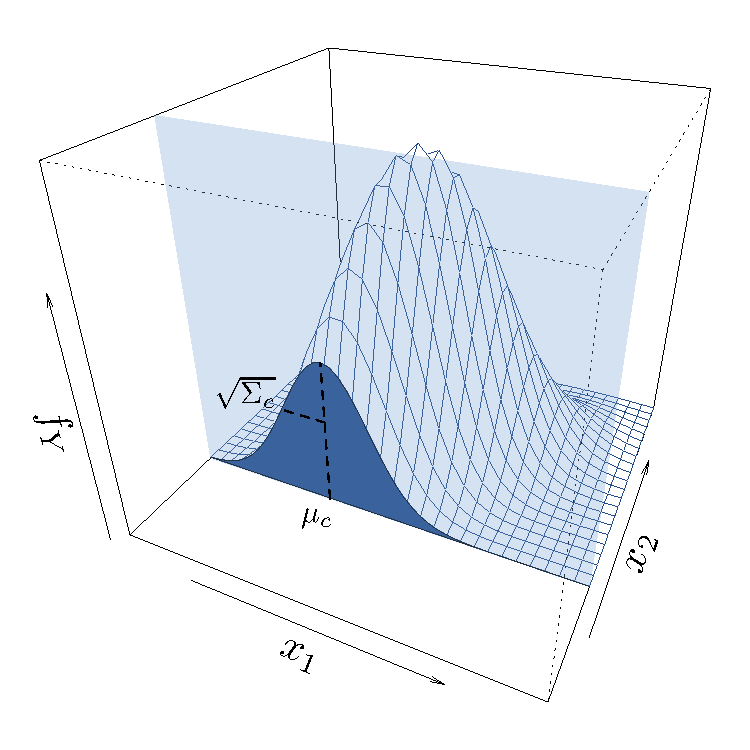
\includegraphics[height=6cm]{figures/ch1_condpdf1}
\end{center}
\end{exampleblock}
\end{frame}

%%%%%%%%%%%%%%%%%%%%%%%%%%%%%%%%%%%%%%%%%%%%%%%%%%%%%%
\begin{frame}{}
\begin{exampleblock}{Example 2}	
3D multivariate Gaussian conditional distribution:\\ 
\begin{center}
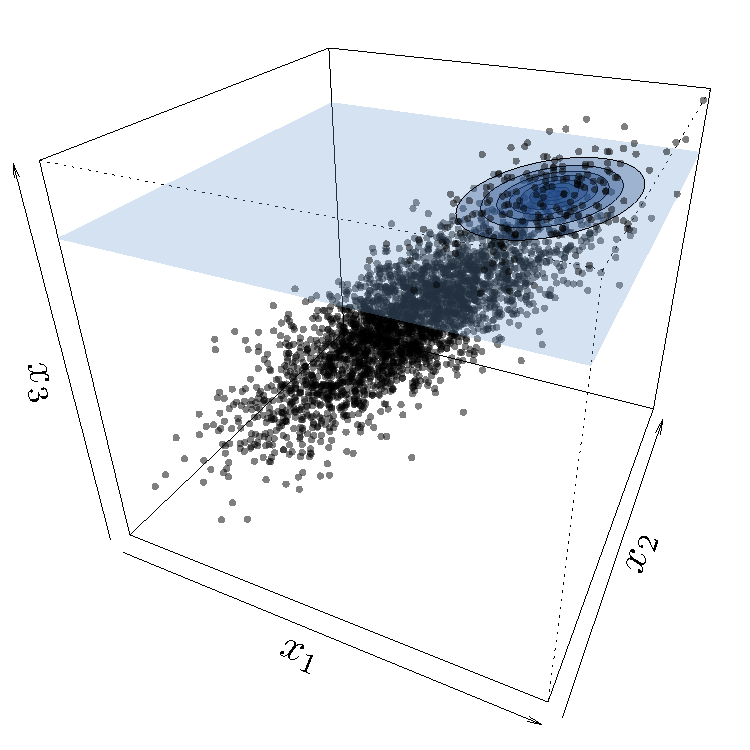
\includegraphics[height=6cm]{figures/ch1_condpdf2} 
\end{center}
\end{exampleblock}
\end{frame}


%%%%%%%%%%%%%%%%%%%%%%%%%%%%%%%%%%%%%%%%%%%%%%%%%%%%%%
\begin{frame}{}
\begin{exampleblock}{Exercise}
	Starting from the density function, prove the previous property using the Schur bloc inverse:
\begin{equation*}
\begin{pmatrix}
	\Sigma_{1,1} & \Sigma_{1,2}\\
	\Sigma_{2,1} & \Sigma_{2,2}\\
\end{pmatrix}^{-1} = 
\begin{pmatrix}
	A & B\\
	B^t & C\\
\end{pmatrix}
\end{equation*}
\begin{equation*}
\begin{split}
 \text{where: \quad} A &= (\Sigma_{1,1} - \Sigma_{1,2} \Sigma_{2,2}^{-1} \Sigma_{2,1})^{-1}\\
 B &= -(\Sigma_{1,1} - \Sigma_{1,2} \Sigma_{2,2}^{-1} \Sigma_{2,1})^{-1}\Sigma_{1,2}\Sigma_{2,2}^{-1}\\
 C &= \Sigma_{2,2}^{-1} + \Sigma_{2,2}^{-1} \Sigma_{2,1} (\Sigma_{1,1} -\Sigma_{1,2} \Sigma_{2,2}^{-1} \Sigma_{2,1})^{-1}\Sigma_{1,2}\Sigma_{2,2}^{-1}
\end{split}
\end{equation*}
\end{exampleblock}
\end{frame}

%%%%%%%%%%%%%%%%%%%%%%%%%%%%%%%%%%%%%%%%%%%%%%%%%%%%%%%%%%%%
%\subsection{Gaussian processes}

%%%%%%%%%%%%%%%%%%%%%%%%%%%%%%%%%%%%%%%%%%%%%%%%%%%%%%
\begin{frame}{2. Gaussian processes}
The multivariate Gaussian distribution can be generalised to random processes: 
\begin{definition}
A random process $Z$ over $D \subset \mathds{R}^d$ is said to be Gaussian if 
\begin{equation*}
\forall n \in \mathds{N}, \forall x_i \in D, (Z(x_1),\dots,Z(x_n)) \text{  is a Gaussian vector}.
\end{equation*} 
\end{definition}
The distribution of a GP is fully characterised by:
\begin{itemize}
	\item its mean function $m$ defined over $D$ 
	\item its covariance function (or kernel) $k$ defined over $D \times D$: $k(x,y) = \Cov(Z(x),Z(y))$
\end{itemize}
We will use the notation $Z \sim \mathcal{N}(m(.),k(.,.))$.
\end{frame}

%%%%%%%%%%%%%%%%%%%%%%%%%%%%%%%%%%%%%%%%%%%%%%%%%%%%%%
\begin{frame}{}
A kernel satisfies the following properties:
\begin{itemize}
	\item It is symmetric: $k(x,y) = k(y,x)$
	\item It is positive semi-definite (psd):
\end{itemize}
\begin{equation*}
	\forall n \in \mathds{N}, \forall x_i \in D, \forall \alpha \in \mathds{R}^n,\  \sum_{i=1}^n \sum_{j=1}^n \alpha_i \alpha_j k(x_i,x_j) \geq 0
\end{equation*}
\vspace{5mm} \\
Furthermore any symmetric psd function can be seen as the covariance of a Gaussian process. This equivalence is known as the Loeve theorem.
\end{frame}

%%%%%%%%%%%%%%%%%%%%%%%%%%%%%%%%%%%%%%%%%%%%%%%%%%%%%%
\begin{frame}{}
Proving that a function is psd is often intractable. However there are a lot of functions that have already been proven to be psd:\\
\vspace{2mm}
\footnotesize
\begin{tabular}{rlN}
		constant & $ \displaystyle k(x,y) = 1 $ &\\[4mm]
		white noise & $ \displaystyle k(x,y) = \delta_{x,y} $ &\\[4mm]
		Brownian & $ \displaystyle k(x,y) =  \min (x,y) $ &\\[4mm]
		exponential & $\displaystyle k(x,y) = \exp \left(- |x-y| \right)$ &\\[4mm]
		Matern 3/2 & $\displaystyle k(x,y) = \left(1 + |x-y| \right) \exp \left(- |x-y| \right)$ &\\[4mm]
		Matern 5/2 & $\displaystyle k(x,y) = \left(1 + |x-y| + 1/3|x-y|^2 \right) \exp \left(- |x-y| \right)$ &\\[4mm]
		squared exponential & $\displaystyle k(x,y) = \exp \left(- (x-y)^2 \right)$ &\\[4mm]
		$\vdots$ & 
		% linear & $ \displaystyle k(x,y) = \sigma^2 xy $ &\\[4mm]
		% cosine & $ \displaystyle k(x,y) = \sigma^2 \cos \left (\frac{x-y}{\theta} \right) $ &\\[4mm]
		% sinc & $ \displaystyle k(x,y) = \sigma^2 \frac{\theta}{x-y} \sin \left( \frac{x-y}{\theta} \right) $ &\\[4mm] \hline
\end{tabular}\\
\vspace{2mm}
\normalsize
When $k$ is a function of $x-y$, the kernel is called \textbf{stationary}.
\end{frame}

%%%%%%%%%%%%%%%%%%%%%%%%%%%%%%%%%%%%%%%%%%%%%%%%%%%%%%
\begin{frame}{}
Can we look at the sample paths associated to these kernels?\\
\vspace{5mm}
In order to simulate sample paths from a GP $Z \sim \mathcal{N}(m(.),k(.,.))$, we will consider samples of the GP discretised on a fine grid.
\vspace{5mm}
\begin{exampleblock}{Exercise: Simulating sample paths}
Let X be a set 100 regularly spaced points over the input space of $Z$.
\begin{itemize}
	\item What is the distribution of $Z(X)$ ?
	\item How to simulate samples from $Z(X)$ ?
\end{itemize}
\end{exampleblock}
\vspace{5mm}
$\Rightarrow$ Shiny App
\end{frame}

%%%%%%%%%%%%%%%%%%%%%%%%%%%%%%%%%%%%%%%%%%%%%%%%%%%%%%
\begin{frame}{}
Furthermore, we can include some scaling parameters into the kernels:
\begin{exampleblock}{Exercise:}
If $Z$ is a GP $\mathcal{N}(0,k(.,.))$, what is the distribution of $Y(x) = \sigma Z(x/\theta)$ ?
\end{exampleblock}
\vspace{5mm}
$\sigma^2$ is called the \textbf{variance} and $\theta$ the \textbf{length-scale}
\end{frame}

%%%%%%%%%%%%%%%%%%%%%%%%%%%%%%%%%%%%%%%%%%%%%%%%%%%%%%
\begin{frame}{}
\begin{exampleblock}{Exercise: }
The kernel is Matern 5/2. Can you put each line in the right order?
\begin{center}
\begin{tabular}{ccc}
$(\sigma^2,\theta) = (3,3)$& $(\sigma^2,\theta)=(1,0.5)$& $(\sigma^2,\theta)=(1,50)$ \\ 
&&\\
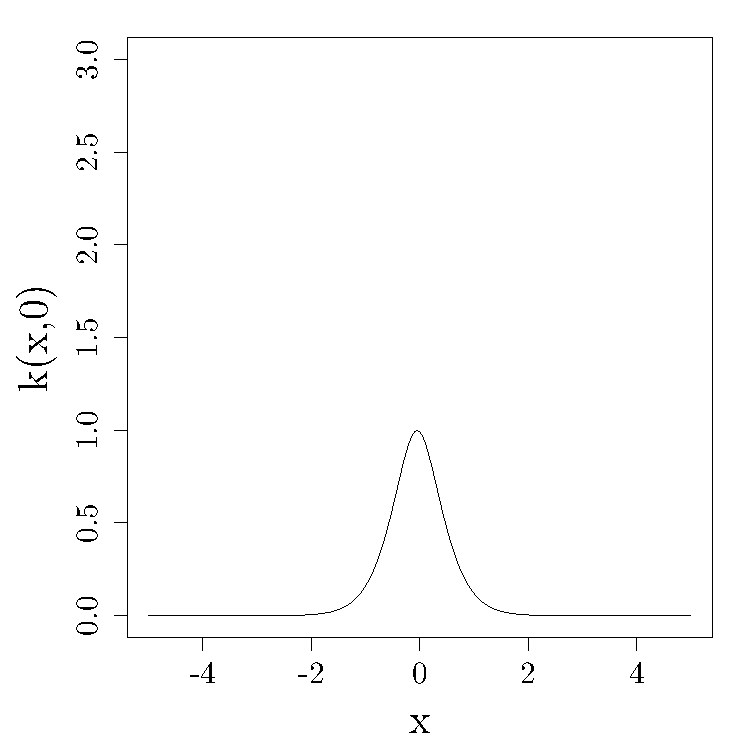
\includegraphics[height=3cm]{figures/R/MVN_kern105} &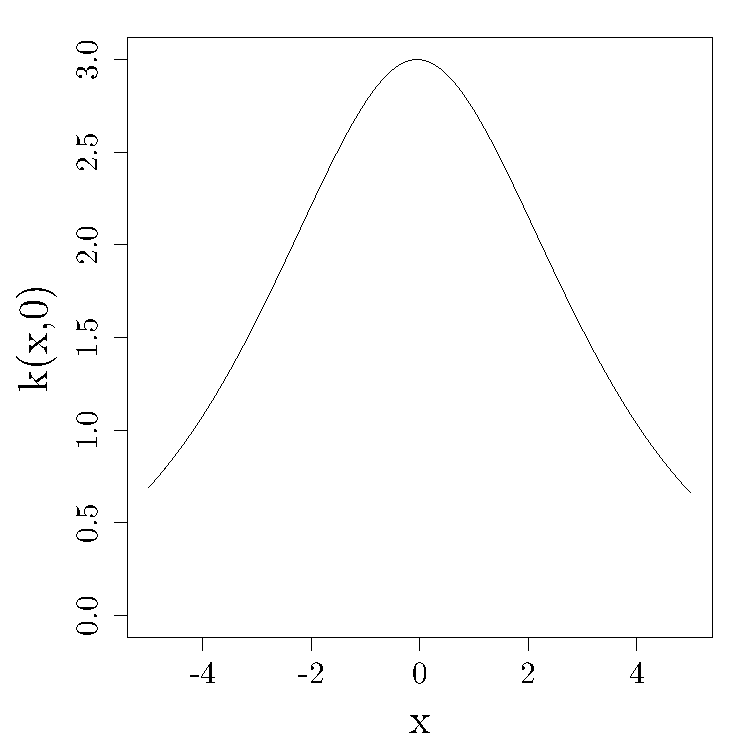
\includegraphics[height=3cm]{figures/R/MVN_kern33}& 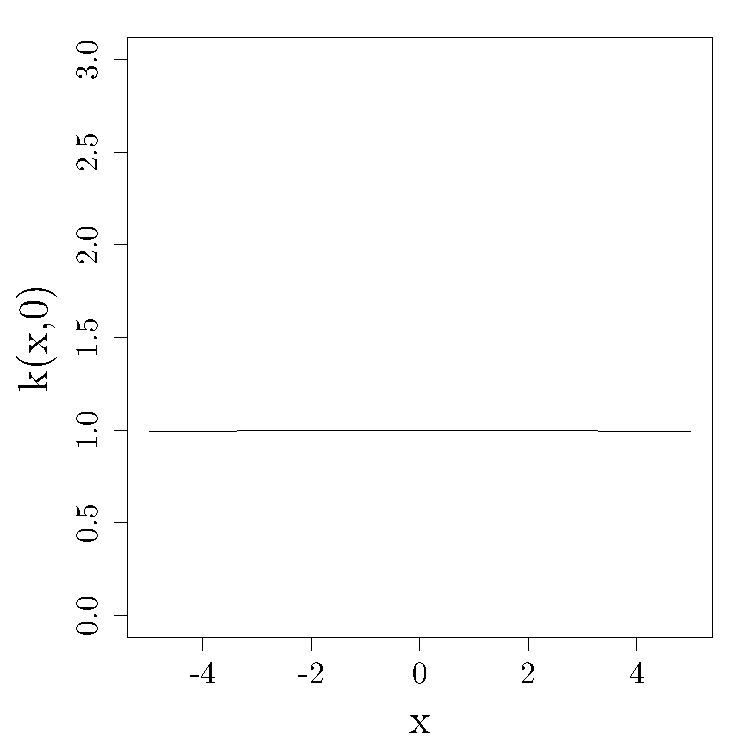
\includegraphics[height=3cm]{figures/R/MVN_kern150}\\ 
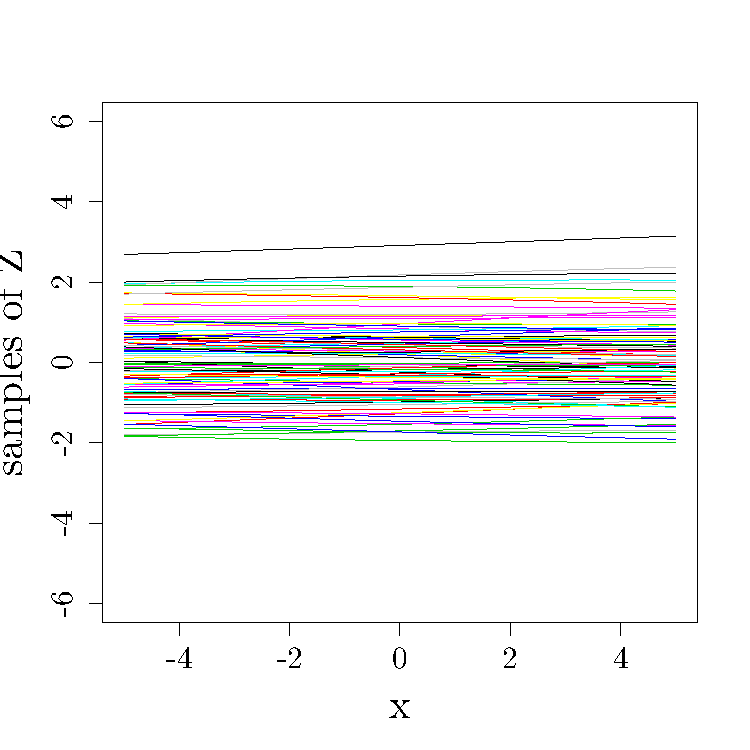
\includegraphics[height=3cm]{figures/R/MVN_traj150} &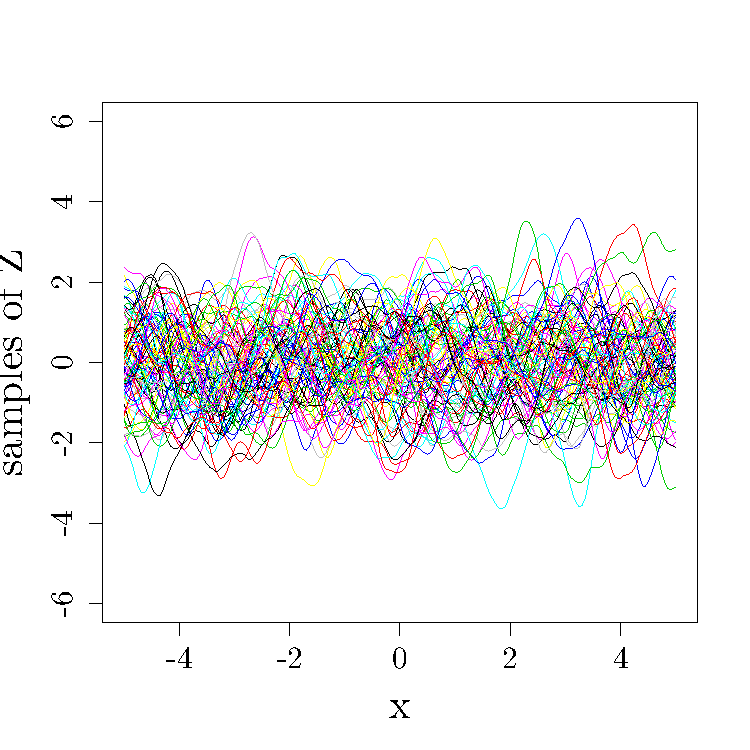
\includegraphics[height=3cm]{figures/R/MVN_traj105}& 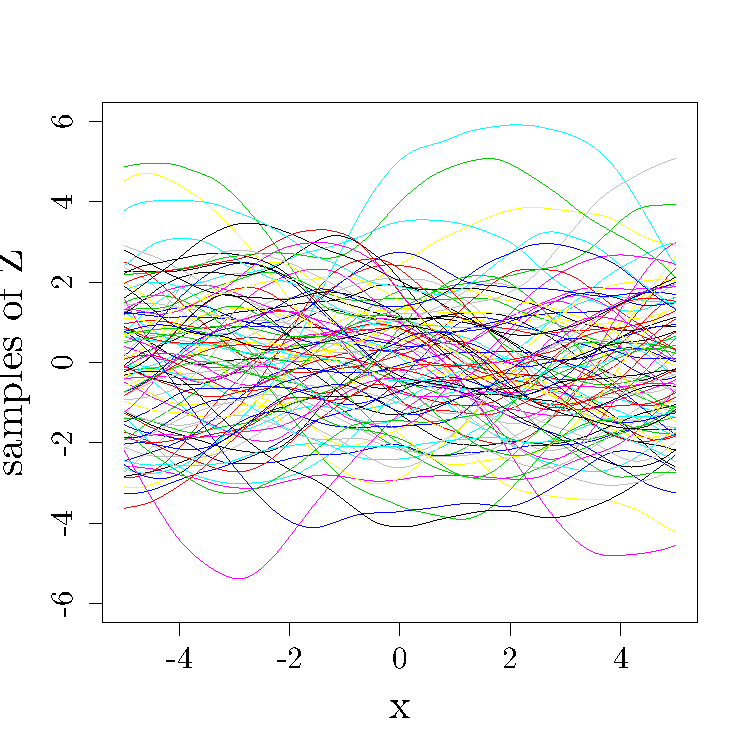
\includegraphics[height=3cm]{figures/R/MVN_traj33}
\end{tabular}
\end{center}
\end{exampleblock}
\end{frame}

%%%%%%%%%%%%%%%%%%%%%%%%%%%%%%%%%%%%%%%%%%%%%%%%%%%%%%
\begin{frame}{}
\begin{exampleblock}{Exercise: }
Answer is:
\begin{center}
\begin{tabular}{ccc}
$(\sigma^2,\theta) = (3,3)$& $(\sigma^2,\theta)=(1,0.5)$& $(\sigma^2,\theta)=(1,50)$ \\ 
&&\\
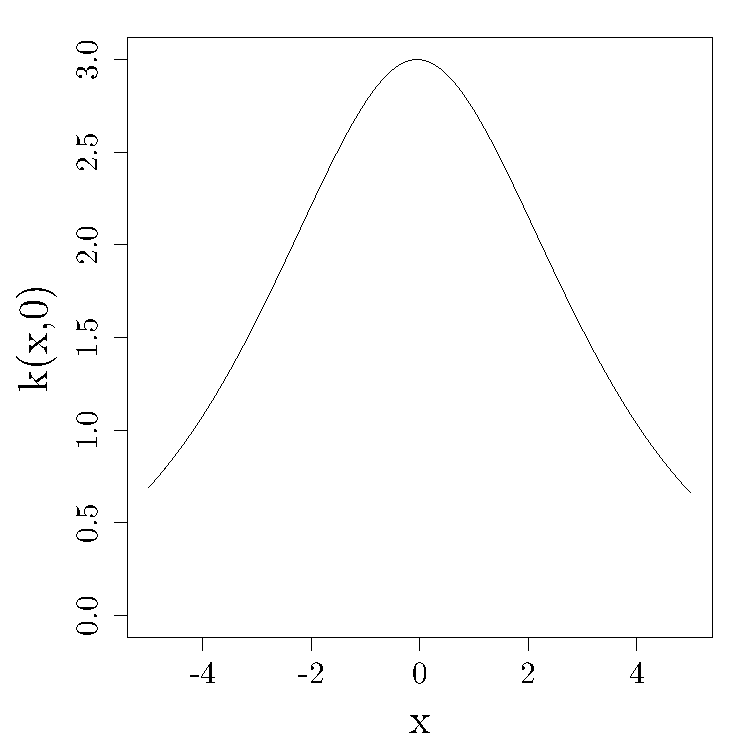
\includegraphics[height=3cm]{figures/R/MVN_kern33} &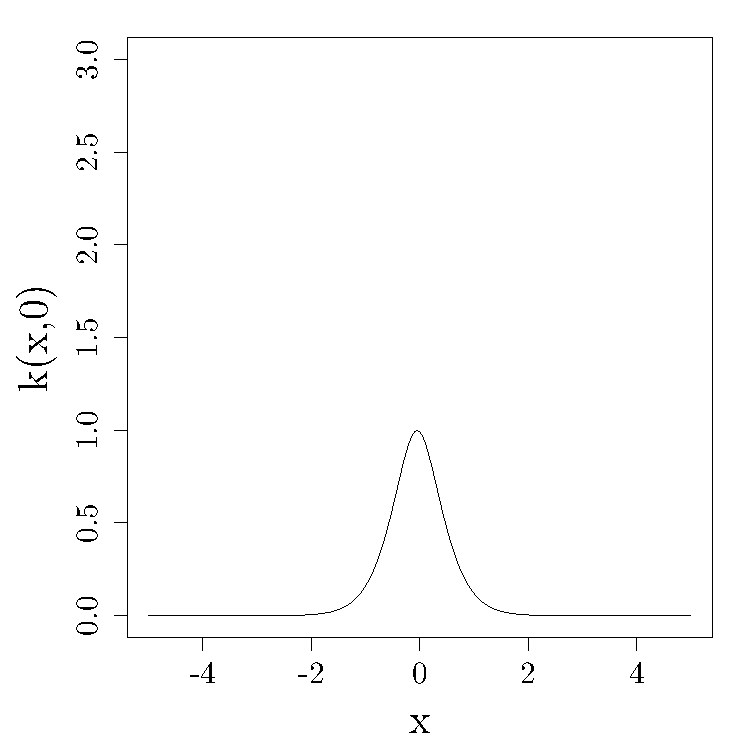
\includegraphics[height=3cm]{figures/R/MVN_kern105}& 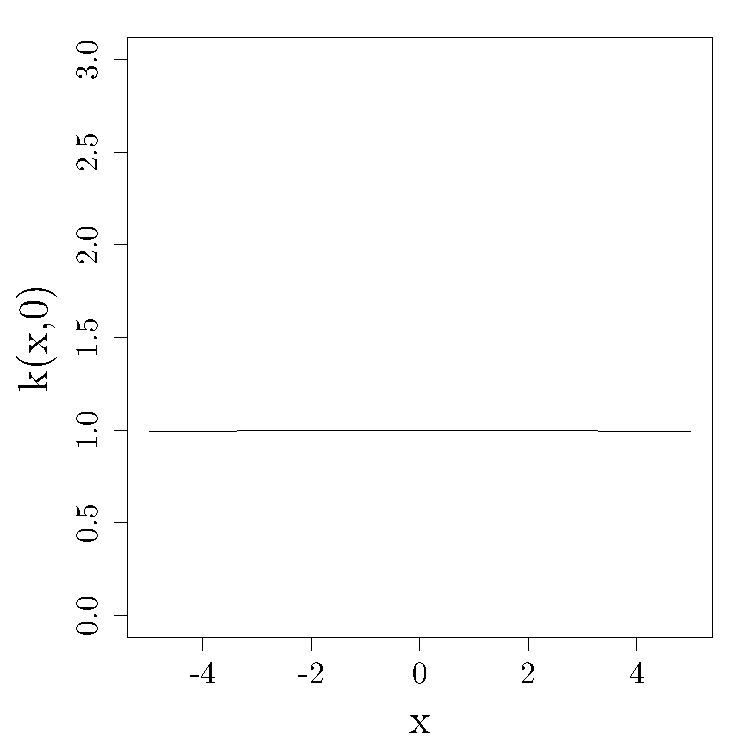
\includegraphics[height=3cm]{figures/R/MVN_kern150}\\ 
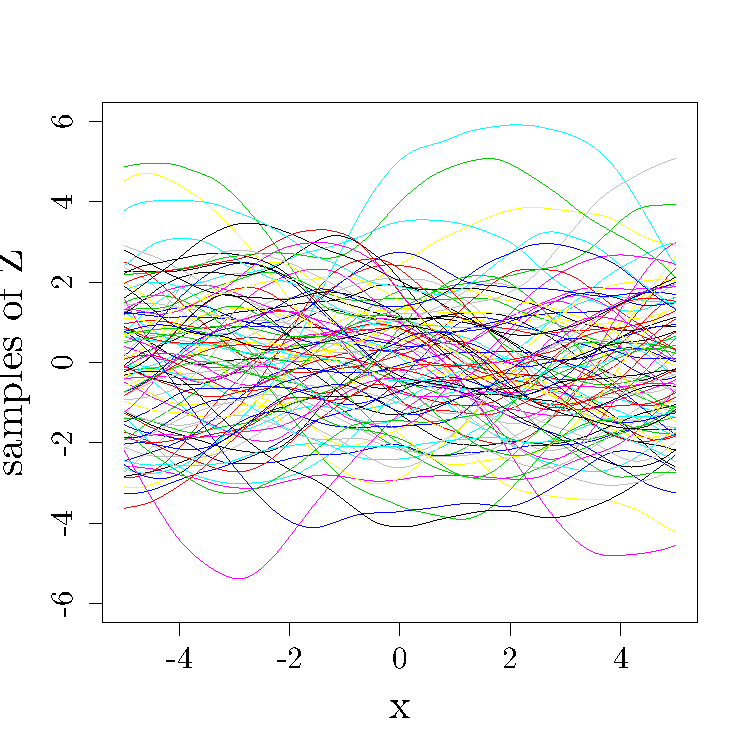
\includegraphics[height=3cm]{figures/R/MVN_traj33} &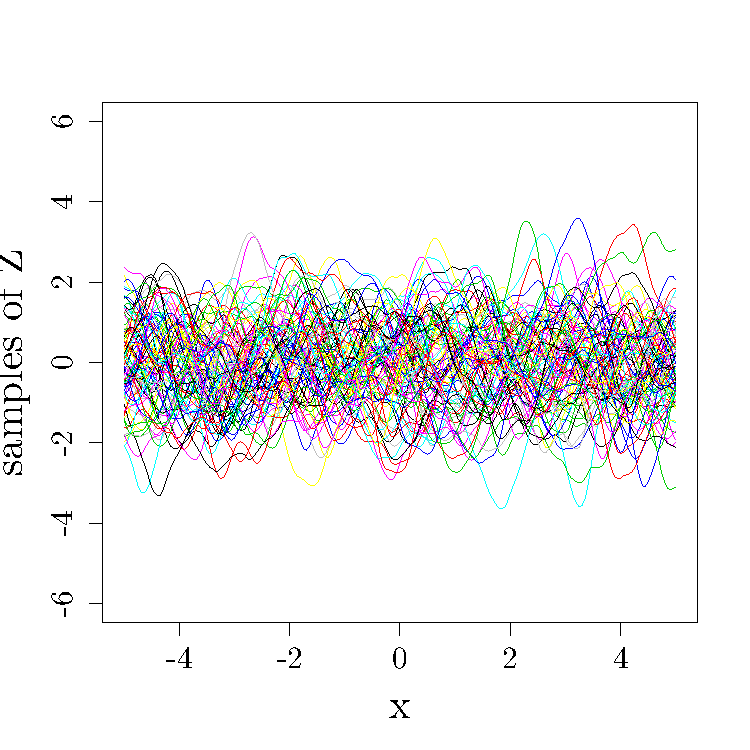
\includegraphics[height=3cm]{figures/R/MVN_traj105}& 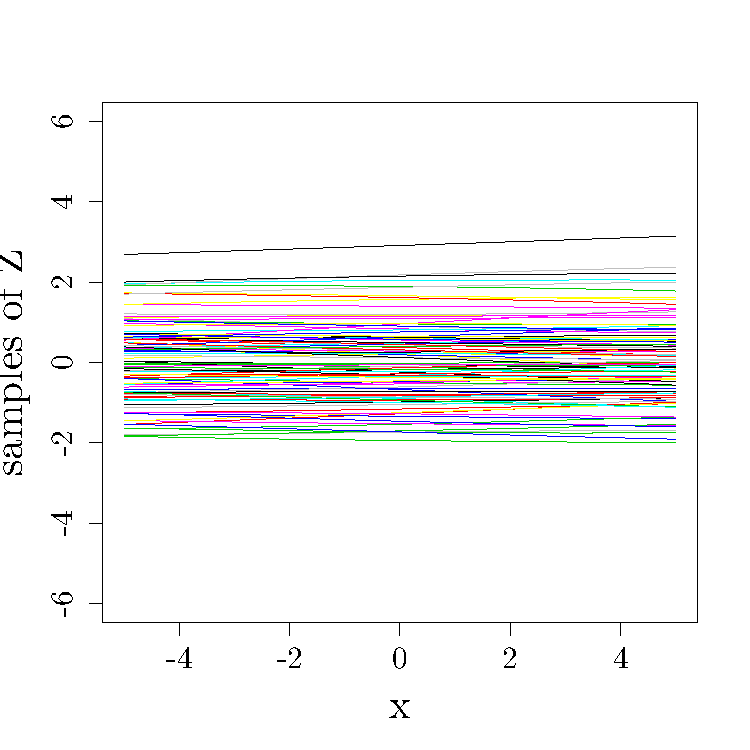
\includegraphics[height=3cm]{figures/R/MVN_traj150}
\end{tabular}
\end{center}
\end{exampleblock}
\end{frame}

%%%%%%%%%%%%%%%%%%%%%%%%%%%%%%%%%%%%%%%%%%%%%%%%%%%%%%
\begin{frame}{}
In higher dimension one can introduce one length-scale parameter per dimension. The usual Euclidean distance between two points $|| x-y || = ( \sum (x_i-y_i)^2)^{1/2}$ is thus replaced by
\begin{equation*}
	\Ni{x-y}{\theta} = \left( \sum_{i=1}^d \frac{(x_i-y_i)^2}{\theta_i^2} \right)^{1/2}.
\end{equation*}
If the parameters $\theta_i$ are equal for all the dimensions, the covariance (or the process) is called \textbf{isotropic}.
\end{frame}

%%%%%%%%%%%%%%%%%%%%%%%%%%%%%%%%%%%%%%%%%%%%%%%%%%%%%%
\begin{frame}{}
Here is a list of the most common kernels:\\
\vspace{2mm}
\footnotesize
\centering
\begin{tabular}{rlN}
		constant & $ \displaystyle k(x,y) = \sigma^2 $ &\\[4mm]
		white noise & $ \displaystyle k(x,y) = \sigma^2 \delta_{x,y} $ &\\[4mm]
		exponential & $\displaystyle k(x,y) = \sigma^2 \exp \left(- \Ni{x-y}{\theta} \right)$ &\\[4mm]
		Matern 3/2 & $\displaystyle k(x,y) = \sigma^2 \left(1 + \sqrt{3}\Ni{x-y}{\theta} \right) \exp \left(- \sqrt{3}\Ni{x-y}{\theta}  \right)$ &\\[4mm]
		Matern 5/2 & $\displaystyle k(x,y) = \sigma^2 \left(1 + \sqrt{5}\Ni{x-y}{\theta} + \frac{5}{3}\Ni{x-y}{\theta}^2 \right) \exp \left(- \sqrt{5}\Ni{x-y}{\theta} \right)$ &\\[4mm]
		Gaussian & $\displaystyle k(x,y) = \sigma^2 \exp \left(- \frac12 \Ni{x-y}{\theta}^2 \right)$ &\\[4mm]
\end{tabular}
\end{frame}

%%%%%%%%%%%%%%%%%%%%%%%%%%%%%%%%%%%%%%%%%%%%%%%%%%%%%%%%%%%%
%\subsection{Gaussian process regression}

%%%%%%%%%%%%%%%%%%%%%%%%%%%%%%%%%%%%%%%%%%%%%%%%%%%%%%
\begin{frame}{3. Gaussian process regression}
We assume we have observed a function $f$ for a set of points $X = (X_1,\dots,X_n)$:
\begin{center}
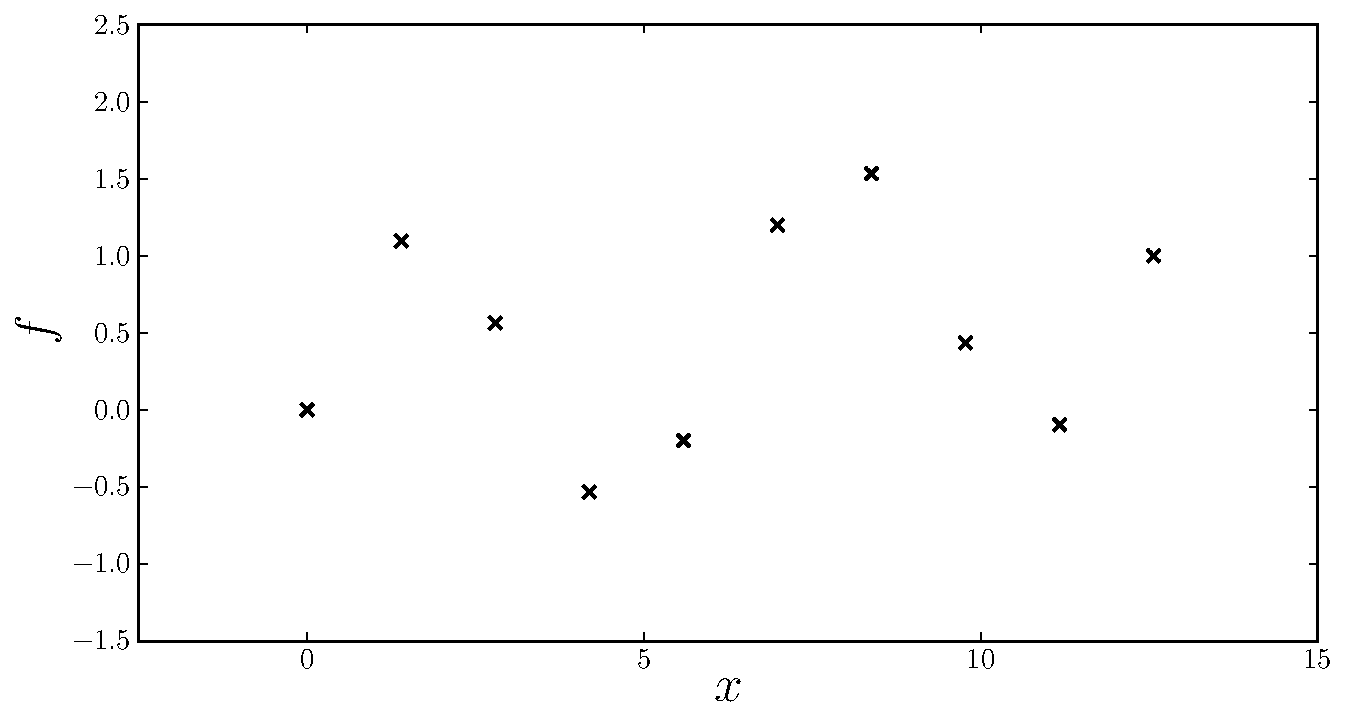
\includegraphics[height=5cm]{figures/R/Fig1-data}
\end{center}
The vector of observations is $F=f(X)$ (ie $F_i = f(X_i)$ ).
\end{frame}

%%%%%%%%%%%%%%%%%%%%%%%%%%%%%%%%%%%%%%%%%%%%%%%%%%%%%%
\begin{frame}{}
Since $f$ in unknown, we make the general assumption that
it is the sample path of a Gaussian process $Z \sim \mathcal{N}(0,k)$:
\begin{center}
\includegraphics[height=5cm]{figures/R/Fig1b-sim}
\end{center}
What would be the next step? 
\end{frame}

%%%%%%%%%%%%%%%%%%%%%%%%%%%%%%%%%%%%%%%%%%%%%%%%%%%%%%
\begin{frame}{}
We can look at the conditional distribution of $Z$ knowing that it interpolates the data points: 
\begin{exampleblock}{Exercise}
\begin{itemize}
	\item[1.] What is the conditional distribution of $Z(x)|Z(X)=F$?
	\item[2.] Compute the conditional mean $m$ and covariance $c(.,.)$.
	\item[3.] Compute $m(X_1)$ and $c(X_1,X_1)$.
\end{itemize}
\end{exampleblock}
\end{frame}

%%%%%%%%%%%%%%%%%%%%%%%%%%%%%%%%%%%%%%%%%%%%%%%%%%%%%%
\begin{frame}{}
\begin{exampleblock}{Solution}
	\begin{itemize}
		\item[1.] The conditional distribution is Gaussian.
		\item[2.] It has mean and variance
			\begin{equation*}
			\begin{split}
				m(x) &= \E[Z(x)|Z(X) \shorteq F] \\
				&= k(x,X) k(X,X)^{-1} F \\ \vspace{3mm}
				c(x,y) &= \Cov[Z(x),Z(y)|Z(X) \shorteq F] \\
				&= k(x,y) - k(x,X) k(X,X)^{-1} k(X,y)
			\end{split}
			\end{equation*}
		\item[3.] We have $m(X_1)=F_1$ and $c(X_1,X_1)=0$
		\end{itemize}
\end{exampleblock}
\end{frame}


%%%%%%%%%%%%%%%%%%%%%%%%%%%%%%%%%%%%%%%%%%%%%%%%%%%%%%
\begin{frame}{}
We can look at sample paths from the conditional distribution 
\begin{center}
\includegraphics[height=6cm]{figures/R/Fig1-sim-cond}
\end{center}
\end{frame}

%%%%%%%%%%%%%%%%%%%%%%%%%%%%%%%%%%%%%%%%%%%%%%%%%%%%%%
\begin{frame}{}
It can summarized by a mean function and 95\% confidence intervals. 
\begin{center}
\includegraphics[height=6cm]{figures/R/Fig1-GP}
\end{center}
\end{frame}

%%%%%%%%%%%%%%%%%%%%%%%%%%%%%%%%%%%%%%%%%%%%%%%%%%%%%%
\begin{frame}{}
A few remarkable properties of GPR models 
\begin{itemize}
	\item They (can) interpolate the data-points
	\item The prediction variance does not depend on the observations
	\item The mean predictor does not depend on the variance
	\item They (usually) come back to zero when we are far away from the observations.
\end{itemize}
Can you prove them?
\end{frame}


%%%%%%%%%%%%%%%%%%%%%%%%%%%%%%%%%%%%%%%%%%%%%%%%%%%%%%
\begin{frame}{}
Changing the kernel \alert{has a huge impact on the model}:\\ 
\vspace{5mm}
\begin{center}
\includegraphics[height=3.9cm]{figures/Fig2-GP-rbf} \qquad 
\includegraphics[height=3.9cm]{figures/Fig2-GP-exp}
\end{center}
\end{frame}

%%%%%%%%%%%%%%%%%%%%%%%%%%%%%%%%%%%%%%%%%%%%%%%%%%%%%%
\begin{frame}{}
This is because changing the kernel means changing the prior on $f$\\ 
\vspace{5mm}
\begin{center}
\includegraphics[height=3.8cm]{figures/Fig2-sim-rbf} \qquad 
\includegraphics[height=3.8cm]{figures/Fig2-sim-exp}
\end{center}
\end{frame}

%%%%%%%%%%%%%%%%%%%%%%%%%%%%%%%%%%%%%%%%%%%%%%%%%%%%%%
\begin{frame}{}
There is no model/kernel that is intrinsically better... it depends on the data!
\begin{center}
\includegraphics[height=3.5cm]{figures/Fig2-GP-rbf} \hspace{1cm}
\includegraphics[height=3.5cm]{figures/Fig2-GP-exp}
\end{center}
The kernel has to be chosen accordingly to our prior belief on the behaviour of the function to study:
\begin{itemize}
  \item is it continuous, differentiable, how many times?
  \item is it stationary ?
  \item ...
\end{itemize}
\end{frame}

%%%%%%%%%%%%%%%%%%%%%%%%%%%%%%%%%%%%%%%%%%%%%%%%%%%%%%
\begin{frame}{}
The best predictor can be seen either as a linear combination of
\begin{itemize}
	\item the observations: $m(x)=\alpha^t F$
	\item the kernel evaluated at $X$: $m(x)=k(x,X) \beta$
\end{itemize} 
The later is interesting to understand the model shape and behaviour. \\
\vspace{5mm}
For example, we have for a squared exponential kernel
\begin{center}
\includegraphics[height=4cm]{figures/R/ch34_basisfuncGauss}  
\includegraphics[height=4cm]{figures/R/ch34_GPRbasisfuncGauss} 
\end{center}
\end{frame}

%%%%%%%%%%%%%%%%%%%%%%%%%%%%%%%%%%%%%%%%%%%%%%%%%%%%%%
\begin{frame}{}
and for a Brownian kernel:
\begin{center}
\includegraphics[height=4cm]{figures/R/ch34_basisfuncBrown}
\includegraphics[height=4cm]{figures/R/ch34_GPRbasisfuncBrown}
\end{center}
\end{frame}

%%%%%%%%%%%%%%%%%%%%%%%%%%%%%%%%%%%%%%%%%%%%%%%%%%%%%%
\begin{frame}{}
We are not always interested in models that interpolate the data. For example, if there is some observation noise: $F = f(X) + \varepsilon$.
% \begin{equation*}
% 	F = f(X) + \varepsilon
% \end{equation*}
% What would change in the model expression?
% \end{frame}

% %%%%%%%%%%%%%%%%%%%%%%%%%%%%%%%%%%%%%%%%%%%%%%%%%%%%%%
% \begin{frame}{}
\vspace{5mm}
Let $N$ be a process $\mathcal{N}(0,n)$ that represent the observation noise. The expressions of GPR with noise are 
\begin{equation*}
	\begin{split}
	m(x) &= \E[Z(x)|Z(X) + N(X) \shorteq F] \\
	&= k(x,X) (k(X,X)+n(X,X))^{-1} F \\ 
	& \\
	c(x,y) &= \Cov[Z(x),Z(y)|Z(X)+ N(X) \shorteq F] \\
	&= k(x,y) - k(x,X) (k(X,X)+n(X,X))^{-1} k(X,y)
\end{split}
\end{equation*}
\end{frame}

%%%%%%%%%%%%%%%%%%%%%%%%%%%%%%%%%%%%%%%%%%%%%%%%%%%%%%
\begin{frame}{}
Examples of models with observation noise for $n(x,y)=\tau^2 \delta_{x,y}$:
\begin{center}
\includegraphics[height=3.5cm]{figures/R/ch34_GPRnoise0001} 
\includegraphics[height=3.5cm]{figures/R/ch34_GPRnoise001} 
\includegraphics[height=3.5cm]{figures/R/ch34_GPRnoise01}\\
The values of $\tau^2$ are respectively 0.001, 0.01 and 0.1.
\end{center}
\end{frame}


%%%%%%%%%%%%%%%%%%%%%%%%%%%%%%%%%%%%%%%%%%%%%%%%%%%%%%%%%%%%
\section{Conclusion}
\subsection{}

%%%%%%%%%%%%%%%%%%%%%%%%%%%%%%%%%%%%%%%%%%%%%%%%%%%%%%
\begin{frame}{}
\structure{Three things to remember:}\\ \vspace{3mm}
\begin{itemize}
	\item Statistical models are useful when little data is available. they allow to
	\begin{itemize}
		\item interpolate or approximate functions
		\item Compute quantities of interests (such as mean value, optimum, ...)
		\item Get an error measure
	\end{itemize}
	\item GPR is similar to linear regression but the assumption is much weaker (not a finite dimensional space)
	\item The GPR equations are
	\begin{equation*}
		\begin{split}
			m(x) & = k(x,X)k(X,X)^{-1}F\\
			c(x,y) &= k(x,y) - k(x,X)k(X,X)^{-1}k(X,y)
		\end{split}
	\end{equation*}
\end{itemize}
\end{frame}

%%%%%%%%%%%%%%%%%%%%%%%%%%%%%%%%%%%%%%%%%%%%%%%%%%%%%%
\begin{frame}{}
We still have many things to discuss about such models:
\begin{itemize}
	\item How to choose the observation points?
	\item How to validate the model?
	\item How to estimate the model (ie kernel) parameters?
\end{itemize}
This will be discussed during the next courses.\\
\vspace{10mm}
\structure{Reference}\\
Carl Edward Rasmussen and Chris Williams, \emph{Gaussian processes for machine learning}, MIT Press, 2006. (free version online).
\end{frame}


%%%%%%%%%%%%%%%%%%%%%%%%%%%%%%%%%%%%%%%%%%%%%%%%%%%%%%%%%%%%%%%%%%%%%%%%%%%%%%%
%%%%%%%%%%%%%%%%%%%%%%%%%%%%%%%%%%%%%%%%%%%%%%%%%%%%%%%%%%%%%%%%%%%%%%%%%%%%%%%
%%%%%%%%%%%%%%%%%%%%%%%%%%%%%%%%%%%%%%%%%%%%%%%%%%%%%%%%%%%%%%%%%%%%%%%%%%%%%%%
%%%%%%%%%%%%%%%%%%%%%%%%%%%%%%%%%%%%%%%%%%%%%%%%%%%%%%%%%%%%%%%%%%%%%%%%%%%%%%%
\end{document}













%%%%%%%%%%%%%%%%%%%%%%%%%%%%%%%%%%%%%%%%%%%%%%%%%%%%%%
%%%%%%%%%%%%%%%%%%%%%%%%%%%%%%%%%%%%%%%%%%%%%%%%%%%%%%
%%%%%%%%%%%%%%%%%%%%%%%%%%%%%%%%%%%%%%%%%%%%%%%%%%%%%%

\structure{}

\begin{center}
  \begin{tabular}{|c|cc|}

  \end{tabular}
\end{center}

###
%%%%%%%%%%%%%%%%%%%%%%%%%%%%%%%%%%%%%%%%%%%%%%%%%%%%%%
\begin{frame}{}

\end{frame}

###
\begin{block}{}

\end{block}

###
\begin{center}
\includegraphics[height=5cm]{figures/}
\end{center}

###
\begin{columns}[c]
\column{5cm}

\column{5cm}

\end{columns}
